\documentclass[11pt,a4paper,oneside]{report}             % Single-side
%\documentclass[11pt,a4paper,twoside,openright]{report}  % Duplex

%\PassOptionsToPackage{chapternumber=Huordinal}{magyar.ldf}
\usepackage{t1enc}
\usepackage[latin2]{inputenc}
\usepackage{amsmath}
\usepackage{amssymb}
\usepackage{enumerate}
\usepackage[thmmarks]{ntheorem}
\usepackage{graphics}
\usepackage{epsfig}
\usepackage{listings}
\usepackage{color}
%\usepackage{fancyhdr}
\usepackage{lastpage}
\usepackage{anysize}
\usepackage[magyar]{babel}
\usepackage{sectsty}
\usepackage{setspace}  % Ettol a tablazatok, abrak, labjegyzetek maradnak 1-es sorkozzel!
\usepackage[hang]{caption}
\usepackage{hyperref}

%--------------------------------------------------------------------------------------
% Main variables
%--------------------------------------------------------------------------------------
\newcommand{\vikszerzo}{Kem�ny K�roly}
\newcommand{\vikkonzulens}{dr. Strausz Gy�rgy}
\newcommand{\vikcim}{Mesters�ges neur�lis h�l�zatok fejleszt�se TensorFlow alapon}
\newcommand{\viktanszek}{M�r�stechnika �s Inform�ci�s Rendszerek Tansz�k}
\newcommand{\vikdoktipus}{Szakdolgozat}
\newcommand{\vikdepartmentr}{B�dis-Szomor� Andr�s}

%--------------------------------------------------------------------------------------
% Page layout setup
%--------------------------------------------------------------------------------------
% we need to redefine the pagestyle plain
% another possibility is to use the body of this command without \fancypagestyle
% and use \pagestyle{fancy} but in that case the special pages
% (like the ToC, the References, and the Chapter pages)remain in plane style

\pagestyle{plain}
%\setlength{\parindent}{0pt} % �ttekinthet�bb, angol nyelv� dokumentumokban jellemz�
%\setlength{\parskip}{8pt plus 3pt minus 3pt} % �ttekinthet�bb, angol nyelv� dokumentumokban jellemz�
\setlength{\parindent}{12pt} % magyar nyelv� dokumentumokban jellemz�
\setlength{\parskip}{0pt}    % magyar nyelv� dokumentumokban jellemz�

\marginsize{35mm}{25mm}{15mm}{15mm} % anysize package
\setcounter{secnumdepth}{0}
\sectionfont{\large\upshape\bfseries}
\setcounter{secnumdepth}{2}
\singlespacing
\frenchspacing

%--------------------------------------------------------------------------------------
%	Setup hyperref package
%--------------------------------------------------------------------------------------
\hypersetup{
    bookmarks=true,            % show bookmarks bar?
    unicode=false,             % non-Latin characters in Acrobat�s bookmarks
    pdftitle={\vikcim},        % title
    pdfauthor={\vikszerzo},    % author
    pdfsubject={\vikdoktipus}, % subject of the document
    pdfcreator={\vikszerzo},   % creator of the document
    pdfproducer={Producer},    % producer of the document
    pdfkeywords={keywords},    % list of keywords
    pdfnewwindow=true,         % links in new window
    colorlinks=true,           % false: boxed links; true: colored links
    linkcolor=black,           % color of internal links
    citecolor=black,           % color of links to bibliography
    filecolor=black,           % color of file links
    urlcolor=black             % color of external links
}

%--------------------------------------------------------------------------------------
% Set up listings
%--------------------------------------------------------------------------------------
\lstset{
	basicstyle=\scriptsize\ttfamily, % print whole listing small
	keywordstyle=\color{black}\bfseries\underbar, % underlined bold black keywords
	identifierstyle=, 					% nothing happens
	commentstyle=\color{white}, % white comments
	stringstyle=\scriptsize\sffamily, 			% typewriter type for strings
	showstringspaces=false,     % no special string spaces
	aboveskip=3pt,
	belowskip=3pt,
	columns=fixed,
	backgroundcolor=\color{lightgray},
} 		
\def\lstlistingname{lista}	

%--------------------------------------------------------------------------------------
%	Some new commands and declarations
%--------------------------------------------------------------------------------------
\newcommand{\code}[1]{{\upshape\ttfamily\scriptsize\indent #1}}

% define references
\newcommand{\figref}[1]{\ref{fig:#1}.}
\renewcommand{\eqref}[1]{(\ref{eq:#1})}
\newcommand{\listref}[1]{\ref{listing:#1}.}
\newcommand{\sectref}[1]{\ref{sect:#1}}
\newcommand{\tabref}[1]{\ref{tab:#1}.}

\DeclareMathOperator*{\argmax}{arg\,max}
%\DeclareMathOperator*[1]{\floor}{arg\,max}
\DeclareMathOperator{\sign}{sgn}
\DeclareMathOperator{\rot}{rot}
\definecolor{lightgray}{rgb}{0.95,0.95,0.95}

\author{\vikszerzo}
\title{\viktitle}
\includeonly{
	guideline,%
	project,%
	titlepage,%
	declaration,%
	abstract,%
	introduction,%
	tensorflow,%
	neural_image_classification,%
	own_work, %
	measurements, %
	chapter3,%
	acknowledgement,%
	appendices,%
}
%--------------------------------------------------------------------------------------
%	Setup captions
%--------------------------------------------------------------------------------------
\captionsetup[figure]{
%labelsep=none,
%font={footnotesize,it},
%justification=justified,
width=.75\textwidth,
aboveskip=10pt}

\renewcommand{\captionlabelfont}{\small\bf}
\renewcommand{\captionfont}{\footnotesize\it}

%--------------------------------------------------------------------------------------
% Table of contents and the main text
%--------------------------------------------------------------------------------------
\begin{document}
\singlespacing
%--------------------------------------------------------------------------------------
% Rovid formai es tartalmi tajekoztato
%--------------------------------------------------------------------------------------

\footnotesize
\begin{center}
\large
\textbf{\Large �ltal�nos inform�ci�k, a diplomaterv szerkezete}\\
\end{center}

A diplomaterv szerkezete a BME Villamosm�rn�ki �s Informatikai Kar�n:
\begin{enumerate}
\item	Diplomaterv feladatki�r�s
\item	C�moldal
\item	Tartalomjegyz�k
\item	A diplomatervez� nyilatkozata az �n�ll� munk�r�l �s az elektronikus adatok kezel�s�r�l
\item	Tartalmi �sszefoglal� magyarul �s angolul
\item	Bevezet�s: a feladat �rtelmez�se, a tervez�s c�lja, a feladat indokolts�ga, a diplomaterv fel�p�t�s�nek r�vid �sszefoglal�sa
\item	A feladatki�r�s pontos�t�sa �s r�szletes elemz�se
\item	El�zm�nyek (irodalomkutat�s, hasonl� alkot�sok), az ezekb�l levonhat� k�vetkeztet�sek
\item	A tervez�s r�szletes le�r�sa, a d�nt�si lehet�s�gek �rt�kel�se �s a v�lasztott megold�sok indokl�sa
\item	A megtervezett m�szaki alkot�s �rt�kel�se, kritikai elemz�se, tov�bbfejleszt�si lehet�s�gek
\item	Esetleges k�sz�netnyilv�n�t�sok
\item	R�szletes �s pontos irodalomjegyz�k
\item	F�ggel�k(ek)
\end{enumerate}

Felhaszn�lhat� a k�vetkez� oldalt�l kezd�d� \LaTeX-Diplomaterv sablon dokumentum tartalma. 

A diplomaterv szabv�nyos m�ret� A4-es lapokra ker�lj�n. Az oldalak t�k�rmarg�val k�sz�ljenek (mindenhol 2.5cm, baloldalon 1cm-es k�t�ssel). Az alap�rtelmezett bet�k�szlet a 12 pontos Times New Roman, m�sfeles sork�zzel.

Minden oldalon - az els� n�gy szerkezeti elem kiv�tel�vel - szerepelnie kell az oldalsz�mnak.

A fejezeteket decim�lis beoszt�ssal kell ell�tni. Az �br�kat a megfelel� helyre be kell illeszteni, fejezetenk�nt decim�lis sz�mmal �s kifejez� c�mmel kell ell�tni. A fejezeteket decim�lis al�oszt�ssal sz�mozzuk, maxim�lisan 3 al�oszt�s m�lys�gben (pl. 2.3.4.1.). Az �br�kat, t�bl�zatokat �s k�pleteket c�lszer� fejezetenk�nt k�l�n sz�mozni (pl. 2.4. �bra, 4.2 t�bl�zat vagy k�pletn�l (3.2)). A fejezetc�meket igaz�tsuk balra, a norm�l sz�vegn�l viszont haszn�ljunk sorkiegyenl�t�st. Az �br�kat, t�bl�zatokat �s a hozz�juk tartoz� c�met igaz�tsuk k�z�pre. A c�m a jel�lt r�sz alatt helyezkedjen el.

A k�peket lehet�leg rajzol� programmal k�sz�ts�k el, az egyenleteket egyenlet-szerkeszt� seg�ts�g�vel �rj�k le (A \LaTeX~ehhez k�zenfekv� megold�sokat ny�jt).

Az irodalomjegyz�k sz�vegk�zi hivatkoz�sa t�rt�nhet a Harvard-rendszerben (a szerz� �s az �vsz�m megad�s�val) vagy sorsz�mozva. A teljes lista n�vsor szerinti sorrendben a sz�veg v�g�n szerepeljen (sorsz�mozott irodalmi hivatkoz�sok eset�n hivatkoz�si sorrendben). A szakirodalmi forr�sok c�meit azonban mindig az eredeti nyelven kell megadni, esetleg z�r�jelben a ford�t�ssal. A list�ban szerepl� valamennyi publik�ci�ra hivatkozni kell a sz�vegben (a \LaTeX-sablon a Bib\TeX~seg�ts�g�vel mindezt automatikusan kezeli). Minden publik�ci� a szerz�k ut�n a k�vetkez� adatok szerepelnek: foly�irat cikkekn�l a pontos c�m, a foly�irat c�me, �vfolyam, sz�m, oldalsz�m t�l-ig. A foly�irat c�meket csak akkor r�vid�ts�k, ha azok nagyon k�zismertek vagy nagyon hossz�ak. Internet hivatkoz�sok megad�sakor fontos, hogy az el�r�si �t el�tt megadjuk az oldal tulajdonos�t �s tartalm�t (mivel a link egy id� ut�n ak�r el�rhetetlenn� is v�lhat), valamint az el�r�s id�pontj�t.

\vspace{5mm}
Fontos:
\begin{itemize}
	\item A szakdolgozat k�sz�t� / diplomatervez� nyilatkozata (a jelen sablonban szerepl� sz�vegtartalommal) k�telez� el��r�s Karunkon ennek hi�ny�ban a szakdolgozat/diplomaterv nem b�r�lhat� �s nem v�dhet� !
	\item Mind a dolgozat, mind a mell�klet maxim�lisan 15 MB m�ret� lehet !
\end{itemize}

\vspace{5mm}
\begin{center}
J� munk�t, sikeres szakdolgozat k�sz�t�st ill. diplomatervez�st k�v�nunk !
\end{center}

\normalsize

%--------------------------------------------------------------------------------------
% Feladatkiiras (a tanszeken atveheto, kinyomtatott valtozat)
%--------------------------------------------------------------------------------------
\clearpage
\begin{center}
\large
\textbf{FELADATKI�R�S}\\
\end{center}

A feladatki�r�st a tansz�ki adminisztr�ci�ban lehet �tvenni, �s a leadott munk�ba eredeti, tansz�ki pecs�ttel ell�tott �s a tansz�kvezet� �ltal al��rt lapot kell belef�zni (ezen oldal \emph{helyett}, ez az oldal csak �tmutat�s). Az elektronikusan felt�lt�tt dolgozatban m�r nem kell beleszerkeszteni ezt a feladatki�r�st.





\pagenumbering{arabic}
\onehalfspacing
%--------------------------------------------------------------------------------------
%	The title page
%--------------------------------------------------------------------------------------
\begin{titlepage}
\begin{center}

\includegraphics[width=60mm,keepaspectratio]{figures/BMElogo.png}\\
\vspace{0.3cm}
\textbf{Budapesti M�szaki �s Gazdas�gtudom�nyi Egyetem}\\
\textmd{Villamosm�rn�ki �s Informatikai Kar}\\
\textmd{\viktanszek}\\[5cm]

\vspace{0.4cm}
{\huge \bfseries \vikcim}\\[0.8cm]
\vspace{0.5cm}
\textsc{\Large \vikdoktipus}\\[4cm]

\begin{tabular}{ccc}
 \makebox[4cm]{\emph{K�sz�tette}} & \makebox[4cm]{\emph{Konzulens}} & \makebox[4cm]{\emph{K�ls� Konzulens}}\\
 \makebox[4cm]{\vikszerzo} & \makebox[4cm]{\vikkonzulens} & \makebox[4cm]{Dar�czy B�lint}
\end{tabular}

\vfill
{\large \today}
\end{center}
\end{titlepage}



\tableofcontents\vfill
%--------------------------------------------------------------------------------------
% Nyilatkozat
%--------------------------------------------------------------------------------------
\begin{center}
\large
\textbf{HALLGAT�I NYILATKOZAT}\\
\end{center}

Alul�rott \emph{\vikszerzo}, szigorl� hallgat� kijelentem, hogy ezt a szakdolgozatot/ diplomatervet \textcolor{blue}{(nem k�v�nt t�rlend�)} meg nem engedett seg�ts�g n�lk�l, saj�t magam k�sz�tettem, csak a megadott forr�sokat (szakirodalom, eszk�z�k stb.) haszn�ltam fel. Minden olyan r�szt, melyet sz� szerint, vagy azonos �rtelemben, de �tfogalmazva m�s forr�sb�l �tvettem, egy�rtelm�en, a forr�s megad�s�val megjel�ltem.

Hozz�j�rulok, hogy a jelen munk�m alapadatait (szerz�(k), c�m, angol �s magyar nyelv� tartalmi kivonat, k�sz�t�s �ve, konzulens(ek) neve) a BME VIK nyilv�nosan hozz�f�rhet� elektronikus form�ban, a munka teljes sz�veg�t pedig az egyetem bels� h�l�zat�n kereszt�l (vagy autentik�lt felhaszn�l�k sz�m�ra) k�zz�tegye. Kijelentem, hogy a beny�jtott munka �s annak elektronikus verzi�ja megegyezik. D�k�ni enged�llyel titkos�tott diplomatervek eset�n a dolgozat sz�vege csak 3 �v eltelte ut�n v�lik hozz�f�rhet�v�.

\begin{flushleft}
\vspace*{1cm}
Budapest, \today
\end{flushleft}

\begin{flushright}
 \vspace*{1cm}
 \makebox[7cm]{\rule{6cm}{.4pt}}\\
 \makebox[7cm]{\emph{\vikszerzo}}\\
 \makebox[7cm]{hallgat�}
\end{flushright}
\thispagestyle{empty}

\vfill
\clearpage
\thispagestyle{empty} % an empty page


%----------------------------------------------------------------------------
% Abstract in hungarian
%----------------------------------------------------------------------------
\chapter*{Kivonat}\addcontentsline{toc}{chapter}{Kivonat}

Jelen dokumentum egy diplomaterv sablon, amely formai keretet ad a BME Villamosm�rn�ki �s Informatikai Kar�n v�gz� hallgat�k �ltal elk�sz�tend� szakdolgozatnak �s diplomatervnek. A sablon haszn�lata opcion�lis. Ez a sablon \LaTeX~alap�, a \emph{TeXLive} \TeX-implement�ci�val �s a PDF-\LaTeX~ford�t�val m�k�d�k�pes.
\vfill

%----------------------------------------------------------------------------
% Abstract in english
%----------------------------------------------------------------------------
\chapter*{Abstract}\addcontentsline{toc}{chapter}{Abstract}

This document is a \LaTeX-based skeleton for BSc/MSc~theses of students at the Electrical Engineering and Informatics Faculty, Budapest University of Technology and Economics. The usage of this skeleton is optional. It has been tested with the \emph{TeXLive} \TeX~implementation, and it requires the PDF-\LaTeX~compiler.
\vfill


%----------------------------------------------------------------------------
\chapter*{Bevezet�}\addcontentsline{toc}{chapter}{Bevezet�}
%----------------------------------------------------------------------------

\section{Motiv�ci�}

\paragraph{A neur�lis h�l�zat} A neur�lis h�l�zat egy sz�m�t�si modell amelyet sz�mos, algoritmikailag neh�z probl�m�ra sikeresen lehet alkalmazni. A f� alkalmaz�si ter�leteik: oszt�lyoz�si feladatok, regresszi�s feladatok, dimenzi� cs�kkent�s �s jellemz� kiemel�s. Ezt a modellt sikeresen alkalmazt�k m�r az ipar sz�mos ter�let�n, a teljess�g ig�nye n�lk�l: 
\begin{enumerate}
\item \emph{k�pfelismer�s:} Ezen a ter�leten tal�n a legsokr�t�bb a felhaszn�l�suk az egyszer� OCR rendszerekt�l kezdve eg�szen a r�kos daganatok detekt�l�s�ig elterjedtek. 
\item \emph{id�sor el�rejelz�s:} Komplex id�sor el�rejelz�sn�l is el�szeretettel haszn�lj�k �ket, amikor a sok v�ltoz�t �s azoknak �sszef�gg�s�t bonyolults�gukn�l fogva m�r nem lehet klasszikus statisztikai m�dszerekkel megragadni.
\item \emph{besz�dszintetiz�l�s:} A 2016 szeptember�ben publik�lt WaveNet strukt�ra 50\%-ot volt k�pes jav�tani Mean Opinion Scoreban az eddigi state-of-the-art besz�dszintetiz�l� rendszereken. Ezt a javul�st nyelvf�ggetlen�l, angolban �s mandarin k�naiban is k�pes volt tartani. \cite{waveNet}
\item \emph{szab�lyoz� algoritmusok:} Szint�n 2016-ban a DeepMind AI alkalmaz�sa a Google egy adatk�zpontj�nak a h�t�s vez�rl�s�ben 40\%-os es�st eredm�nyezett az erre ford�tott kiad�sokban.
\end{enumerate}
Ezek v�lem�nyem szerint mind kifejezetten izgalmas eredm�nyek, tiszt�n l�tszik hogy a ter�let �l, fejl�dik �s napr�l napra form�lja a jelfeldolgoz�sr�l alkotott k�p�nket.

\paragraph{Jelen Dolgozat c�lja} A dolgozat f� csap�sir�nya egy �ttekint� k�p alkot�sa a neur�lis h�l�zatok felhaszn�l�s�r�l k�poszt�lyoz�si probl�m�k eset�ben. A dolgozatomban arra t�rekszem hogy a neur�lis h�l�zatok gyakorlati alkalmaz�s�t ezen az alter�leten kereszt�l ismerjem meg. Mivel tanulm�nyaim sor�n ilyesf�le - matematikai vonatkoz�s� - programoz�ssal nem tal�lkoztam jelent�s m�rt�kben, ez�rt ez egy j� alkalom arra hogy l�ssam hogy komplex matematikai absztrakci�k hogyan �ltenek testet szoftverk�nt. P�ld�ul a sztochasztikus generativ vagy a konvoluci�s neur�lis h�l�zatok hogyan ford�that�ak le effekt�v programm�, �s hogyan lehet bel�l�k �rt�kes alkalmaz�sokat k�sz�teni. A szakdolgozat egy hosszabb projekt r�sze, ahol egy Tegra mobil chipen kell majd k�poszt�lyz� algoritmusokat alkalmazni ami egy robotrep�l�g�pen fog val�s idej� d�nt�seket hozni. A dolgozat �r�sa alatt �rt�kel�dik ki hogy a projektben a Tensorflow re�lis alternat�va lesz-e a tov�bbi munk�hoz, illetve hogy melyik k�poszt�lyz� elj�r�s felelne meg legjobban a c�ljainknak.

\paragraph{�rdekl�d�sem a neur�lis h�l�zatok ir�nt} Az �n�ll� labor munk�m sor�n �s a szakir�nyomon oktatott kooperat�v �s tanul� rendszerek t�rgyban tal�lkoztam el�sz�r ezzel a megk�zel�t�ssel. Az egyre modernebb aj�nl� algoritmusok keres�se k�zepedte r� kellett eszm�lnem hogy az aj�nl�rendszerek j�v�je is �sszefon�dik a neur�lis h�l�zatok�val. Am�g a 2015�s RecSys konferenci�n egyetlen papir sem sz�lt a m�ly tanul�sr�l, az idei konferencia publik�ci�inak a negyede a m�ly modellek felhaszn�l�s�t taglalta. Igy ez a dolgozat hab�r els� l�t�sra nem is l�tszik, de az �n�ll� laborat�riumi projekt munk�m tov�bbvitele. Egy potenci�lisan �rdekes, m�g alig kutatott ter�let, hogy a term�kek hib�s �s hi�nyos le�r�s�t hogyan lehet augment�lni a term�kek felt�lt�tt k�peib�l kinyert c�mke felh�vel. Erre nagy val�sz�n�s�ggel alkalmazhat� h�l�zatok lenn�nek a region�lis konvoluci�s h�l�zatok amiket �rint�legesen t�rgyalok majd a konvuluci�s h�l�zatokat taglal� fejezetben.

\paragraph{A feladat indokolts�ga} Az olvas� jogosan teheti fel mag�ban a k�rd�st hogy ha ezek a h�l�zatok m�r l�teznek, s�t sok esetben konfigur�ci� n�lk�l "out of the box" jelleggel haszn�lhat�ak, akkor mi ad l�tjogosults�got egy ilyen bevezet� jelleg� szakdolgozatnak? Nos, hab�r az el�z� pont igaz, m�gis manaps�g minn�l ink�bb �rdemes tiszt�ban lenni ezeknek az eszk�z�knek a k�pess�geivel, �s mind fontosabb a korl�taival. Ha valaki egy saj�t alkalmaz�sban szeretn� �ket haszn�lni, akkor �rdemes tudni hogy:
\begin{enumerate}
\item \ Az adott alkalmaz�shoz milyen h�l� t�pusok haszn�lhat�ak.
\item \ Van-e esetleg m�r el�re tan�tott modell a feladatunkhoz. 
\item \ Ha nincs akkor mennyi id� lenne betan�tani egyet.
\item \ Mennyi mem�ri�t �s sz�m�t�st ig�nyelnek az egyes modellek. (Ez er�sen p�ld��l f�gg a modell param�ter ter�nek nagys�g�t�l)
\end{enumerate}
A szakdolgozat v�g�re rem�nyeim szerint az egyetemi t�rgyak anyag�t tov�bbfejlesztve egy nagyobb r�l�t�ssal fogok rendelkezni erre az izgalmas ter�letre.

\paragraph{A dolgozat kontextusa} Ahhoz hogy kontextusba helyezem jelen munk�mat a bevezet� tov�bbi r�sz�ben szeretn�k egy r�vid �ttekint�st adni a g�pi tanul�s t�rt�nelm�r�l.

\section{A g�pi tanul�s igen r�vid t�rt�nelme}

\begin{enumerate}
\item \ Az els� elismerten tanul� g�pet Arthur Samuelnek tulajdon�tj�k 1955-ben, ez a konstrukci� k�pes volt megtanulni d�maj�t�kot j�tszani. Samuel algoritmusai heurisztikus keres�si mem�ri�t alkalmaztak annak �rdek�ben hogy a saj�t tapasztalataikb�l tanuljanak. A hetvenes �vek k�zep�re ez a rendszer m�r k�pes volt emberi j�t�kosok legy�z�s�re is.
\item \ K�vetkez� fontos pontk�nt Frank Rosenblatt Perceptronj�t emeln�m ki, ez volt az els� neur�lis h�l�zat, 1958-ban alkotta meg Rosenblatt az amerikai haditenger�szet "US office of Naval Research" laborat�rium�ban. M�r ezt is vizu�lis mint�k felismer�s�re alkott�k meg eredetileg.
\item \ A hetvenes �veket csak �gy emlegetik hogy a mesters�ges intelligencia tele, miut�n Marvin Minksy 1969-ben r�mutatott a Perceptron korl�taira az emberek elvesztett�k az �rdekl�d�s�ket a ter�let ir�nt.
1985-ben egy forradalmi �j�t�s, a hibavisszaterjeszt�ses algoritmus (backpropagation algorithm \cite{backProp}) t�rte meg a csendet �s keltette fel az emberek �rdekl�d�s�t �jfent ezen sz�m�t�si strukt�r�k ir�nt. 
\item \ A kilencvenes �vekben a neur�lis h�l�zatok �jra kiker�ltek a k�z�ppontb�l, mert a statisztikusok �ltal alkotott szupport vektor g�pek (tov�bbiakban SVM) l�nyegesen jobb teljes�m�nyt tudtak el�rni, kevesebb tan�t�ssal mint a kor h�l�zatai.
\item \ A neur�lis h�l�zatok k�vetkez� vir�gkor�t napjainkban �lj�k, ennek egyik f� t�nyez� a fejlett neur�lis strukt�r�k felfedez�se, illetve az hogy a grafikus egys�gek �s a sz�m�t�si f�rt�k fejl�d�s�nek k�sz�nhet�en eddig elk�pzelhetetlen sz�m�t�si kapac�t�s �ll rendelkez�s�nkre a h�l�zataink tan�t�s�ra. Ezzel szemben a kernel g�peken alapul� modellek nem tudtak a megn�vekedett teljes�tm�nyt kihaszn�lva a neur�lis h�l�zatokhoz hasonl� pontoss�g n�veked�st el�rni. A manaps�g a neur�lis h�l�zatok jelen vannak az �let minden ter�let�n ahol sz�ks�g�nk van mint�zatok intelligens felismer�s�re, lehet a t�rgya hang, k�p vagy ak�r sz�veges dokumentumok. Google translate, Shazam, a Netflix d�j nyertes aj�nl�si algoritmus, csak hogy p�r p�ld�t szemelv�nyezzek a sz�mtalan k�z�l.
\end{enumerate}

\paragraph{A dolgozat fel�p�t�se} A dolgozatomat az al�bbi �p�tem fel:
\begin{enumerate}
\item \ A tensorflow mint neur�lis rendszerek kutat�s�ra, fejleszt�s�re �s �les �zembe helyez�s�re alkalmas platform bemutat�sa.
\item \ A t�rgyter�let irodalm�nak �ttekint�se, szeml�zve a k�vetkez� strukt�r�kat:
\begin{enumerate}
\item \ Egyszer� t�bbr�teg� perceptron.
\item \ Korl�tozott boltzmann g�pek, �s vari�nsai
\item \ Konvoluci�s Neur�lis h�l�zatok
\item \ A friss fejlem�nyek a neur�lis k�poszt�lyoz�s ter�let�n.
\end{enumerate}
\item \ A saj�t fejleszt�seim bemutat�sa, amely egy k�t egyszer�bb strukt�ra implement�l�sa �s vizsg�lata a fent bemutatottak k�z�l, a tensorflow k�nyvt�rral.
\item \ A m�r�si eredm�nyeim ki�rt�kel�se, tanuls�gok levon�sa.
\end{enumerate}
%----------------------------------------------------------------------------
\chapter{A Tensorflow\cite{tensorflow} �kosziszt�ma �ttekint�se}

\section{A Tensorflow k�nyvt�r.}

\paragraph{A technol�giai v�laszt�s indokl�sa} A modern szoftverm�rn�ki munka szerves r�sze a rendelkez�sre �ll� eszk�z�k garmad�j�b�l a legmegfelel�bb kiv�laszt�sa. Ez a k�n�lat m�r�t�ke, az inform�ci�k elsz�rts�ga �s ellentmond�soss�ga miatt kor�nt sem egy egyszer� feladat. A c�mb�l tal�n �gy sejlik hogy a tensorflow a munk�mhoz m�r egy el�re eld�nt�tt v�laszt�s volt, de ez a meg�llap�t�s kor�nt sem lenne helyt�ll�. A szakdolgozatom nulladik l�psek�nt sz�mos m�s - a neur�lis h�l�zatok fejleszt�s�t t�mogat� - k�nyvt�rat vettem szem�gyre. A teljess�g ig�nye n�lk�l: Caffee, Chainer, CNTK, Matlab, Tensorflow, Thenao, Torch. A k�vetkez�kben szeretn�m bemutatni az �ltalam v�lasztott eszk�z a Tensorflow fel�p�t�s�t, �s ezzel mintegy implicit m�don megindokolni hogy szerintem mi�rt ez a megfelel� eszk�z a neur�lis h�l�zatokkal val� munk�hoz.

\paragraph{Bevezet�} Munk�m sor�n a Tensorflow nev� k�nyvt�rral dolgoztam. A Tensorflow egy elosztott, sz�m�t�si gr�f alap� numerikus k�nyvt�r. A Goolge Deep Mind kutat�csoport szakemberei hozt�k l�tre azzal a c�llal hogy saj�t modelljeiket fejlessz�k �s �rt�kelj�k ki benne. A k�nyvt�r a DistBelief nev� keretrendszer egyenes�gi lesz�rmazottj�nak tekinthet�. A DistBelief csendben megh�z�dva, de ott dolgozik a fejlett vil�g majdnem minden ember�nek az �lete m�g�tt, l�v�n hogy az Alphabet c�gcsoport (A Google feldarabol�s�nak ut�dv�llalait �sszefog� holding) t�bb mint 50 csapata adapt�lta, �s v�rtezte fel �ltala intelligenci�val alkalmaz�s�t. P�r ismertebbet kiemelve: Google Search, Adwords, Google Maps, SteetView, Youtube, �s term�szetesen a Google Translate. Miut�n �vek tapasztalata gy�lemlet fel az els� gener�ci�s k�nyvt�ruk haszn�lata sor�n, �gy �rezt�k  itt az id� hogy - szak�tva a technol�giai teherrel amit az els� gener�ci� hib�i miatt magukkal hordoztak - l�trehozz�k a k�vetkez� gener�ci�s g�pi tanul�s rendszer�ket, ez lett a Tensorflow aminek a f� c�lja sk�l�zhat�, elosztott g�pi tanul�si algoritmusok (f�k�pp neur�lis h�l�zatok) fejleszt�se.

\paragraph{A Tensorflow alapgondolata.} Mint m�r eml�tettem a Tensorflow k�nyvt�rban az ember a modelljeit egy adatfolyam-szer� sz�m�t�si gr�fk�nt defini�lhatja. Ennek a megk�zel�t�snek az a nagy el�nye hogy nagyon j� sk�l�z�d�si tulajdons�gokkal rendelkezik. Miut�n a gr�f csom�pontjai az egyes sz�m�t�sok, ezek adott esetben hat�kony m�don sz�toszthat�k k�l�nb�z� eszk�z�k, vagy ak�r eg�sz g�pek k�z�tt szerverparkokban. A k�nyvt�r ezen tulajdons�g�nak m�g egy hosszabb r�szt fogunk k�s�bb szentelni.
A l�trej�tt gr�fra mint egy alaprajzra �rdemes gondolni, amit azt�n az egyes munkamenetetek (session-�k) p�ld�nyos�tanak. Ezek a munkamenetek inicializ�lj�k a v�ltoz�kat, �s a munkamenet k�pes a gr�f egyes csom�pontjait lefuttatni, amik ig�ny vez�relt m�don minden a bemenet�kre kapcsol�d� cs�csot lefuttatnak am�g el nem �rnek egy bemenetig vagy egy k�v�lr�l bet�pl�lt v�ltoz�ig. Miut�n a csom�pont sikeresen lefutott a kimenet�t a csatolt nyelv egy v�ltoz�jak�nt adja vissza, p�ld�ul egy Python vagy C++ t�mbk�nt. Fontos megjegyezni hogy fut�s k�zben a gr�ffal nem lehet �rintkezni, az egy atomi egys�gk�nt fut le, hogy minn�l jobban ki lehessen optimaliz�lni a sz�m�t�sokat.

\section{A Tensorflow modellek monitoroz�sa �s hibamentes�t�se}

\paragraph{A Tensorboard} Mivel a modern g�pi tanul�s modellek hihetetlen �sszetetts�ggel b�rnak, �s nagyon sok mozg� alkatr�sz�k van, ez�rt term�szetesen felmer�l az ig�ny hogy egy ilyen �jszer� keretrendszerben ipari er�ss�g� monitoroz� �s hibakeres� funkci�k ker�ljenek bele. Ezeket az elv�r�sokat a Tensorflow eset�ben a mell�kelt Tensorboard alrendszer teljes�ti, amelyet munk�m sor�n �n is extenz�ven haszn�ltam. Ebb�l kifoly�lag most nem is bocs�jtan�m b�vebb t�rgyal�sra, hanem majd az �n�ll� munka szekci�ban ismertetn�m.

\section{A Tensorflow fut�s k�zben} 

\paragraph{A Tensorflow serving kiszolg�l� rendszer} Miut�n a kutat�laborokb�l kiker�ltek az �j g�pi tanul�s modellek nem el�g �ket csak publik�lni, a c�gek komoly hasznot rem�lnek t�l�k. A Google is kijelentette hogy "Information Retrieval first company" helyett �k most m�r egy "AI first company". Ez term�szetesen egy hozz� ill� infrastrukt�ra n�lk�l elk�pzelhetetlen. Ez�rt is hozt�k l�tre a Tensorflowhoz a Tensorflow Servinget, ami egy flexibilis, magas rendelkez�sre �ll�s� kiszolg�l�rendszer. A rendszer lehet�v� teszi �j architekt�r�k kiprob�l�s�t, �zembe helyez�s�t �s A/B tesztel�s�t, mik�zben egy stabil, verzi�zott API-t biztos�t a kliensek sz�m�ra. Term�szetesen ez mit sem �rne ha nem sk�l�zna gond n�lk�l hatalmas magass�gokba, ez�rt egyszer�en integr�lhat� a Kubernetes n�vre hallgat� docker alap� cluster kezel� rendszerrel.

\paragraph{A tensorflow sk�l�zod�sa} �rdemes belegondolni hogy az adatk�zpont TCP (DCTCP) vagy az Infiniband kapcsolatok adott esetben ak�r t�bb gigabyteos sebess�get �rhetnek el, ugyanakkor a m�trix szorz�s - ami a g�pi tanul� algoritmusoknak egy kardin�lis eleme - n�gyzetes ord�t ig�nyel. Teh�t sokkal jobban meg�ri r�szgr�fokat a csom�pontok k�z�tt sz�tosztani �s ink�bb a h�l�zati t�bblettel kalkul�lni, mint hogy egyetlen g�pre b�zzuk a feladatokat.
A m�sik v�gletben viszont egy m�sik elv�r�s helyezkedik el. Miut�n mondjuk egy oszt�lyoz�si feladatn�l a modell�nket megtan�tottuk felismerni valamit, tegy�k fel hogy p�ld�ul egy, a l�t�ss�r�lt embereknek k�sz�tett alkalmaz�sban felismerni az forgalomjelz� l�mp�kat �s azok �llapot�t, term�szetes lenne az ig�ny hogy ezt a r�szorul� mag�val tudja vinni. A h�l� ugyan az, a s�lyokat m�r megtanultuk, de most az eg�sz modell�nket egy mobil eszk�z�n kell futtatni. Ez az eszk�z az inferenci�t j�cint k�nnyeds�ggel b�rn�, csak a tanul�st nem tudtuk volna kivitelezni rajta. M�rn�kk�nt logikus az ig�ny hogy ehhez ne kelljen m�gegyszer lefejleszteni a modell-t, �gy id�t �s p�nzt sp�rolva. Erre lehet�s�g van a keretrendszerrel.

\paragraph{Mobil k�rnyezet} A Tensorflow t�mogatja a mobil eszk�z�n val� fut�st, az el�bbi szcen�ri� a k�nyvt�rral egy teljesen j�rhat� �tt� v�lik. A modell-t asztali sz�m�t�g�pen fejlesztem, adatparkon tan�tom, �s egy mobil eszk�z�n futtatom, mindezt jelent�sebb k�d �jra�r�s n�lk�l. J� p�ld�ja ennek a felhaszn�l�si m�dnak a Google Translate, leg�jabb, nagy felhajt�st el�r� verzi�ja. Ez az alkalmaz�s a nyelvi modelleket a Google irdatlan infrastrukt�r�j�n tanul folyamatosan, mik�zben az inferenci�t a telefonk�sz�l�ken futtatj�k lok�lisan. Itt igaz�ndib�l k�t neur�lis h�l� is szerepet j�sztik, az egyik a sz�veget ismeri fel a k�pen (feltehet�en egy faster R-CNN), a m�sik pedig az effekt�v ford�t�st v�gzi.

%----------------------------------------------------------------------------
\chapter{A Neur�lis h�l�zatokkal val� k�pfeldolgoz�s lehet�s�geinek �ttekint�se}
%----------------------------------------------------------------------------

A kutat�munka egy jelent�s r�sz�t tette ki a dolgozatomnak, mivel az �vek folyam�n nagyon sok sikeres �s sikertelen k�s�rlet sz�letett annak �rdek�ben hogy hogyan lehetne neur�lis h�l�zatokkal k�pi adatokat feldolgozni. Tal�n mondhatjuk hogy ezek a h�l�zatok a legsikeresebb k�poszt�lyoz�, de kor�ntsem trivi�lis hogy mik az el�nyeik, h�tr�nyaik �s az egyes t�pusok milyen komplexit�s� jelekkel k�pesek megb�rk�zni. El�sz�r szeretn�m bemutatni az adathalmazokat amiken ezeket az algoritmusokat ki�rt�kelik, majd eljutni az t�bbr�teg� perceptronokt�l a konvoluci�s h�l�zatokig, v�g�l a leg�jabb trendek ismertet�s�vel z�rni a fejezetet.

\section{Az algoritmusok ki�rt�kel�se}

\subsection{Az adathalmazok}
\paragraph{Bevezet�s} Mint a legt�bb kutat�si ter�letnek, ennek is vannak j�l ismert "benchmark" adathalmazai, amelyek viszony�t�si alapk�nt lehet�s�get biztos�tanak az egym�st�l elt�r� algoritmusok egym�shoz val� ki�rt�kel�s�re. Mivel ezekre az adathalmazokra sokat fogok hivatkozni, ez�rt szeretn�m �ket egy-egy bekezd�sben bemutatni.

\paragraph{MNIST} Az MNIST adatb�zis fekete feh�rt 20x20 pixelre normaliz�lt �rott sz�mjegyeket tartalmaz null�t�l kilencig, azaz t�z oszt�llyal rendelkezik. Az adatb�zis 60'000 annot�lt tan�t� k�pet �s 10'000 annot�lt teszt k�pet tartalmaz. Ez a legalapabb adathalmaz 

\paragraph{CIFAR-10} A CIFAR-10 egy j�val �sszetettebb adathalmaz, 60'0000 annot�lt 32x32 pixeles, sz�nes k�pet tartalmaz. A k�pek 10 oszt�lyra vannak felosztva, oszt�lyonk�nt 6000 k�ppel. Az adathalmazb�l 50'000 k�p van tan�t�sra, �s 10'000 tesztel�sre fenntartva. 

\paragraph{CIFAR-100} A CIFAR-100 fel�p�t�se megegyezik a CIFAR-10el, de oszt�lyrendszere az el�bbin�l l�nyegesen �sszetettebb, 100 oszt�lyt tartalmaz �s minden oszt�lyhoz 600 k�pt tartozik, ezen fel�l m�g 20 �ltal�nosabb oszt�lyba is be vannak sorolva a k�pek, hogy a h�l�zat �ltal�nos�t�s�r�l k�vetkeztet�seket lehessen levonni. P�ld�ul az halak szuperoszt�lyhoz tartozik a r�ja, lazac, stb.

\paragraph{IMAGENET} Az IMAGENET a vil�g legnagyobb k�pgy�jtem�nye, a WordNet lexik�lis adatb�zis szinon�ma halmazai szerint vannak annot�lva a k�pek. Jelenlegi statiszik�i:
\begin{itemize}
\item 14'197'112 annot�lt k�p
\item 21'841 nem �res szinon�ma halmaz
\item 1'034'908 k�p objektumaihoz van m�g hat�rol� doboz annot�ci� is
\item 1'000 szinon�ma halmazhoz tartozik SIFT jellemz�kkel ell�tott k�p
\item 1'200'000 k�p van SIFT jellemz�kkel ell�tva.
\end{itemize}
L�that� hogy az el�z� h�rom adathalmazt az IMAGENET m�r csak puszta m�reteivel is messze t�lsz�rnyalja. Ezt mondhatjuk az etalon benchmarknak. Az �vente megrendezett, a g�pi l�t�s "olimpi�j�nak" sz�m�t� ILSVRC(Large Scale Visual Recognition Challenge) is ezen az adatsokas�gon szokott megrendez�sre ker�lni, jellemz�en 4 kateg�ri�ban: objektum lokaliz�ci�, objektum detekci�, helysz�n felismer�s (pl tengerpart, hegyek), helysz�n meg�rt�s. A legut�bbi nem takar kevesebbet mint egy k�p szemantikus r�szekre val� feloszt�sa, p�ld��l �t, �g, ember vagy �gy.

\subsubsection{A metrika}
\paragraph{MNIST �s CIFAR} Az MNIST �s a CIFAR-10/100 Adathalmazok eset�ben mindig az egyszer� pontoss�g �rt�ket n�zz�k, teh�t az eltal�lt k�pek sz�m�t osztva a hib�san oszt�lyozott k�pet sz�m�val.

\paragraph{IMAGENET} Mivel az IMAGENET egy ennyire bonyolult adathalmaz, itt top 5 hib�t szoktak n�zni, ahol az sz�m�t sikeres tal�latnak ha a helyes c�mket a h�l� 5 legnagyobb val�sz�n�s�ggel b�r� tippj�ben benne van.

\section{A Legelterjedtebb neur�lis h�l�zatok k�pfeldolgoz�shoz}

\paragraph{Bevezet�s} Az �vek sor�n sz�mos neur�lis h�l�zattal k�s�rleteztek a kutat�k annak �rdek�ben hogy r�j�jjenek melyek k�pesek legjobban megtanulni a k�pekeben el�fordul� szab�lyoss�gokat, �s ez alapj�n oszt�lyozni �ket. Ezekb�l szeretn�m a f� �llom�sokat kiemelni, �s le�rni hogy mik voltak a hi�nyoss�gok a megl�v� architekt�r�kban amik �j strukt�r�k l�trehoz�s�t motiv�lt�k. Az �ttekint�sben nem ejtek sz�t a minden h�l�zat t�pusra �rv�nyes �ltal�nos, k�l�nf�le reguraliz�ci�s elj�r�sokr�l, mint a s�lyok felejt�se vagy a dropout met�dus. Csak a h�l�zatok fel�p�t�s�nek �s tan�t�s�nak architekt�r�lis k�l�nbs�geit veszem g�rcs� al�.

\subsection{A t�bbr�teg� perceptron (MLP)}

\subsubsection{Az MLP el�zm�nyei �s megalkot�sa}
\paragraph{El�zm�nyek} Miut�n Rosenblatt megalkotta az els� perceptron strukt�r�t a k�sei �tvenes �vekben, a kutat�k elkezdtek azon gondolkodni hogy hogyan lehetne ezeket a neuronokat �sszerendezni �gy, hogy egy�tt tanuljanak, �s komplex regresszi�k, illetve oszt�lyoz�si feladatok elv�gz�s�re legyenek k�pesek. De ezek a kutat�sok sok�ig igen medd�ek voltak.

\begin{figure}[!ht]
\centering
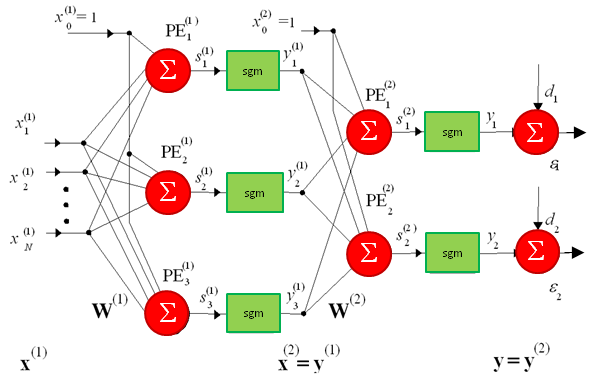
\includegraphics[width=120mm, keepaspectratio]{figures/MLP.png}
\caption{Egy k�tr�teg� MLP h�l�zat.} 
\label{fig:MLP}
\end{figure}

\paragraph{Backpropagation} Az �tt�r�s 1986-ban j�tt, amikor Geoffrey E. Hinton koll�g�ival sikeresen alkalmazta a hibavisszaterjeszt�ses algoritmust az MLP s�lyainak megv�ltoztat�s�ra a n�gyzetes hiba minimaliz�l�s�nak �rdek�ben.
Az algoritmus l�nyege hogy a hib�t a h�l�zatban a deriv�l�s l�nc szab�ly�nak seg�ts�g�vel terjesztj�k vissza. Az algoritmust helymegtakar�t�s �rdek�ben r�szletesebben nem ismertetem, az �rdekl�d�k a bekezd�s elej�n refer�lt cikkben tov�bbi r�szleteket tal�lhatnak. Az algoritmus pseudok�d �sszefoglal�s�t a \figref{MLP}-�br�n 
l�that� h�l�zat tan�t�s�hoz a \listref{Backpropagation}-lista mutatja.

\begin{lstlisting}[frame=single,float=!ht,caption= A backpropagation algoritmus pseudok�dja, label=listing:Backpropagation, mathescape=true]
  inicializ�ljuk a h�l� s�lyait (�ltal�ban 0-1 k�z� es� v�letlen sz�mok)
  do
     forEach tan�t� p�lda legyen tp
        j�solt_c�mke = h�l�-kiement(h�l�, tp)
        val�di_c�mke = tan�t�_c�mke(ex)
        hiba sz�m�t�s f(j�solt_c�mke - val�di_c�mke) minden kimeneti egys�gen
        $\Delta W^{(2)}$ kisz�m�t�sa
        $\Delta W^{(1)}$ kisz�m�t�sa
        a h�l�zat s�lyainak friss�t�se
  until Az �sszes bemenet sikeresen van oszt�lyozva, 
  		vagy m�s meg�ll�si krit�riumot el nem �rt�nk
  return a h�l�zatot
\end{lstlisting}

\subsubsection{Az MLP teljes�tm�nye k�poszt�lyoz�si feladatokra}
\paragraph{Aktiv�t�s a ter�leten.} Gondolhatn�nk hogy ezt a t�m�t m�r r�g elfelejtett�k a kutat�k, de mivel az MLP egy igen egyszer� strukt�ra, ez�rt folyik m�g n�h�ny kutat�s hogy a hat�rait megtal�lj�k.

\paragraph{MNIST} Az MLP teljes�tm�nye k�poszt�lyoz�si feladatok tekitet�ben igen szer�ny a t�bbi h�l�zathoz k�pest, de az MNIST adathalmazzal m�g ez is eg�sz j�l megb�rk�zik, n�h�ny figyelemre m�lt�bb eredm�nyt a \tabref{MLPTablazat}~t�bl�zat foglal �ssze. A t�bbi adathalmazon a naiv MLP nem hoz �rt�kelhet� eredm�nyt, ennek az okait mindj�rt megvizsg�ljuk.

\begin{table}[ht]
	\footnotesize
	\centering
	\caption{Az MLP teljes�tm�nye az MNIST adathalmazon} \label{tab:MLPTablazat}
	\begin{tabular}{ | l | c | c |}
	\hline
	R�tegek sz�ma & neuron strukt�ra & Teszt szet hiba sz�zal�k \\ \hline
	3-r�teg & 768-300-10 & 4.7\\
	\hline
	\end{tabular}
\end{table}

\subsubsection{MLP hi�nyoss�gai} 
Ez az egyetlen eredm�ny amely �rtelmesen �rtelmezhet� a naiv, csak fel�gyelt tan�t�ssal tan�tott MLP tekintet�ben. Ennek sz�mos oka van, ezeket vizsg�lom most meg.

\paragraph{A tanul�s jellege} A fel�gyelt tanul�s kapzsi m�don a hibaf�ggv�nyt a s�lyok gradiens�nek ir�ny�ba optimaliz�lja, ezzel az a probl�ma hogy a hibafel�let egy MLP eset�ben t�bb� nem konvex mint egy egyszer� neuron eset�ben. A bonyolult hibaf�ggv�ny k�vetkezt�ben lok�lis minimumok alakulnak ki. Sok esetben egy j� lok�lis minimumot sem �r�nk el naiv tan�t�ssal, a glob�lis minimum el�r�s�nek az es�lye pedig statisztikailag nulla. Ezt a jelens�get hivatott az al�bb egyszer� f�ggv�ny $\sigma^2(\sigma(x) + \sigma(y))$ kont�r diagrammja (\figref{sigmaContour}~�bra). Ez hab�r nem k�zvetlen�l egy hibaf�ggv�ny, de ezt a tulajdons�g�t j�l szeml�lteti. 

\paragraph{A strukt�ra kialak�t�sa} Az MLP annyira �ltal�nos strukt�r�t haszn�l, hogy l�nyeg�ben semmilyen a priori tud�st nem haszn�lunk fel a h�l�zat tan�t�sakor. Ez azt eredm�nyezi hogy hatalmas kapac�t�s kell a k�pekben megjelen� bonyolult strukt�r�k megtanul�s�hoz. Sajnos az el�bbi c�l csak a h�l�zat n�vel�s�vel �rhet� el, az MLP param�ter tere viszont nagyon rosszl sk�l�z�dik. Ha vesz�nk egy 6 r�teg� h�l�zatot aminek a r�tegjei rendre 2500-2000-1500-1000-500-10 neuronb�l �llnak, �s az MNIST eset�n 784 elem� bemeneti vektorral rendelkezik, akkor optimaliz�land� param�ter t�r m�rete annak folyt�n hogy minden r�teg teljesen �ssze van kapcsolva m�r:
$784 * 2500 + 2500 * 2000 + 2000 * 1500 + 1500 * 1000 + 1000 * 500 + 500 * 10 = 11965000$, ami m�r nyilv�n val�an hatalmas. Ez is tan�that� sikeresen, de ahhoz m�r a tov�bbiakban bemutott kiseg�t� neur�lis strukt�r�k sz�ks�gesek.

\begin{figure}[!ht]
\centering
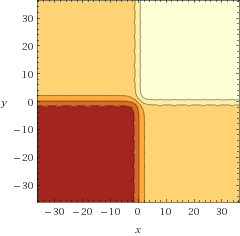
\includegraphics[width=30mm, keepaspectratio]{figures/sigmaContour}
\caption{P�lda egy kompon�lt szigmoid f�ggv�nyre.} 
\label{fig:sigmaContour}
\end{figure}

\subsection{A Korl�tozott Boltzmann G�p}
\paragraph{Bevezet�s} A korl�tozott boltzmann g�p (tov�bbiakban RBM - Restricted Boltzmann Machine, \figref{rbm}~�bra) egy szochasztikus generat�v neur�lis sz�m�t�si modell. M�k�d�se az eddig t�rgyalt MLP-t�l gy�rekesen elt�r, funkci�ja a bemenet jellemz�inek (featureinek) a megtanul�sa, �s nem az egyes mint�k helyes oszt�lyoz�sa. Az intuit�v jelent�s�ge abban rejlik hogy feltehetj�k hogy a na�v MLP a kapzsi tanul�sa miatt nem k�pes megtanulni a mint�k val�di reprezent�ci�j�t, de ha az MLP s�lyait �gy tudn�nk inicializ�lni �gy, hogy a mint�kban l�v� szab�lyoss�gokat m�r eleve ismerje, akkor ebb�l k�nnyebben meg tudja tanulni hogy melyik jellemz� mely oszt�lyt azons�tja.
Ezt fel�gyelt tanul�s el�tti f�zist nem fel�gyelt el�tanul�snak h�vjuk, szok�s m�g erre a c�lra Autoencoder h�l�zatokat haszn�lni, illetve m�ylebb h�l�kra az RBM �s az Autoencoder t�bbr�teg� megfelel�it a m�ly hiedelem h�l�zatokat, �s a "stacked" autoencodereket.
Hab�r a leg�jabb eredm�nyek szerint az Autoencoder hasonl�an j� eredm�nyre vezet, �s kev�sb� bonyolult ez�rt gyakorlatban az aj�nlott, �n m�gis az RBM-et v�lasztottam �rdekes strukt�r�ja miatt. Hugo Larochelle et al. hozott ki egy �ttekint� tanulm�nyt az el�tanul�sr�l a m�lyebben �rdekl�d�knek "Exploring Strategies for Training Deep Neural Networks" \cite{ExploringStrategies} c�mmel.

\paragraph{Az RBM strukt�r�ja} Az RBM mint eml�tettem egy sztochasztikus generat�v sz�m�t�si modell, amelyben fontos hogy az egyes neuronok egy p�ros gr�fot alkotnak (\figref{rbm}~�bra). A generat�v modell egy r�gi statisztik�b�l sz�rmaz� fogalom ami azt foglalja mag�ban hogy a model k�pes megfigyelhet� adatpontokat v�letlenszer�en gener�lni. Az RBM egyik legtrivi�lisabb m�r�sz�ma a rekonstrukci�s hiba azt m�ri hogy ha egy adatpontot a h�l� bemenet�re teszek, akkor azt milyen r�szletesen tudja visszagener�lni. Teh�t az adatpont az a h�l� tanul�si ter�ben egy stabil pontnak sz�m�t-e. Ez a hiba m�rt�k nem j� az RBM �ltal�nos�t� k�pess�g�nek m�r�s�re, m�gis sokan haszn�lj�k praktikus egyszer�s�ge miatt. Akit b�vebben �rdekel a t�ma a \cite{rbmGuide}-es referenci�ban tal�l b�s�ges irodalmat az RBM tan�t�s�t illet�en. Itt csak az alapokra szor�tkozok.

\begin{figure}[!ht]
\centering
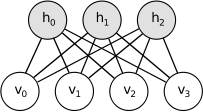
\includegraphics[width=50mm, keepaspectratio]{figures/rbm}
\caption{Egy RBM h�l�zat. Forr�s: \protect\url{http://deeplearning.net/tutorial/_images/rbm.png}} 
\label{fig:rbm}
\end{figure}

\begin{figure}[!ht]
\centering
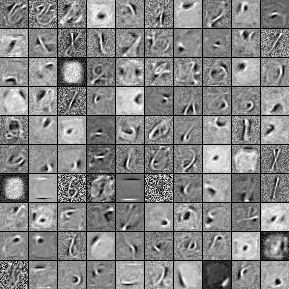
\includegraphics[width=50mm, keepaspectratio]{figures/rbmFilters}
\caption{Egy RBM �ltal megtanult filterek. Forr�s: \protect\url{http://www.pyimagesearch.com/wp-content/uploads/2014/06/rbm_filters.png}} 
\label{fig:rbmFilters}
\end{figure}

\paragraph{Az RBM tan�t�sa} Az RBM az�rt �rdekes megk�zel�t�s a t�bbi h�l�zathoz k�pest, mert probablisztikus alapokon nyugszik. Az �gynevezett energia alap� h�l�zatok felfoghat�ak �gy, hogy a h�l�zat minden konfigur�ci�j�hoz tartozik egy $p(x)$ val�sz�n�s�g, hogy mekkora val�sz�n�s�ggel tart�zkodik a h�l� az adott konfigur�ci�ban. Azt szeretn�nk el�rni hogy az alacsony energi�j� konfigur�ci�knak nagy legyen a val�sz�n�s�ge. Ez formaliz�lva a k�vetkez� k�ppen n�z ki:

\begin{align} \label{probFirst}
p(x) = \frac{e^{(-E(x))}}{Z} = \sum_{h}\frac{e^{(-E(x,h))}}{Z}
\end{align}
\begin{align}
Z = \sum_{x} e^{(-E(x)})
\end{align}

Ahol az E az energiaf�ggv�nyt jelenti. A fizik�ban j�rtasabb olvas�k megfigyelhetik hogy ez a val�sz�n�s�gi f�ggv�ny megfelel a termodinamik�ban haszn�lt Boltzmann eloszl�s val�sz�n�s�gi f�ggv�ny�nek. Az eredeti boltzmann g�pet egy fizikus alkotta meg, pont erre az anal�gi�ra �p�tve, az�rt hogy a Hopfield h�l�zatok gyenges�geit kik�sz�b�lje. A \eqref{probFirst} k�pletet felhaszn�lva megalkothatjuk a hibaf�ggv�ny�nket, amely a negat�v logaritmikus val�sz�n�s�gi f�ggv�ny (negative log likelihood function) lesz:
\begin{align}
\mathcal{L}(\theta, x) = \frac{1}{N}\sum_{x^(i) \in \mathcal{D}}log(p(x^{(i)})
\end{align}

Defini�ljuk a szint�n a temodinamik�b�l sz�rmaz� szabad energia f�ggv�nyt:
\begin{align}
\mathcal{F} = -log\sum_{h}e^{-E(x,h)}
\end{align}

Ezzel �jradefini�lhatjuk a val�sz�n�s�gi f�ggv�nyt:
\begin{align}
p(x) = \frac{e^{-\mathcal{F}(x)}}{Z} \quad \textrm{ahol} \quad Z = \sum_{x}e^{-\mathcal{F}(x)}
\end{align}

Ami megengedi hogy a k�vetkez�t �rhassuk fel:
\begin{align} \label{rbmPFromEnergy}
-\frac{\partial{logp(x)}}{\partial\theta} 
\approx 
\frac{\partial\mathcal{F(x)}}{\partial\theta} - 
\frac{1}{|\mathcal{N}|}
\sum_{\widehat{x} \in \mathcal{N}}
\frac{\partial \widehat{x}}{\partial \theta}
\end{align}

Ha az el�bbi f�ggv�nyt deriv�ljuk, akkor megkapjuk a s�lyv�ltoz�k update f�ggv�ny�t:
\begin{align} \label{RbmWDirect}
-\frac{\partial logp(v)}{\partial W_{ij}} = E_v[p(h_i|v) * v_j] - v_j^{(i)} * sigm(W_i * v^{(i)} + c_i)
\end{align}
\begin{align} \label{RbmCDirect}
-\frac{\partial logp(v)}{\partial c_i} = E_v[p(h_i|v)] - sigm(W_i * v^{(i)})
\end{align}
\begin{align} \label{RbmBDirect}
-\frac{\partial logp(v)}{\partial b_j} = E_v[p(h_i|v) * v_j] - v_j^{(i)}
\end{align}

Ebb�l l�that� hogy az egyes deriv�ltak kisz�m�t�s�hoz sz�ks�g�nk van a rejtett neuronok val�sz�n�s�g�re a bemeneti neuronok �llapot�t�l f�gg�en. Ez�rt sz�ks�ges hogy a boltzman g�p korl�tozott legyen, teh�t egy p�ros gr�p form�j�t vegye fel, mert �gy az egyes neuronokhoz tartoz� val�sz�n�s�gek p�rhuzamos�tva sz�molhat�ak, mivel f�ggetlenek egym�st�l. Erre egy gyors elj�r�s a kontraszt�v divergencia algoritmus amelynek a val�zs�n�s�gi mintav�tel�t a \figref{gibbs}~�bra szeml�lteti. A gibbs mintav�telez�shez tartoz� markov l�nc l�p�seinek a k�pleteit a \eqref{h1} �s a \eqref{v1}~k�plet �rja le.

\begin{align} \label{h1}
h^{n+1} \quad \sim \quad sigm(W^Tv{(n)} + c) 
\end{align}  

\begin{align} \label{v1}
v^{n+1} \quad \sim \quad sigm(W^Th^{(n)} + b) 
\end{align}


\begin{figure}[!ht]
\centering
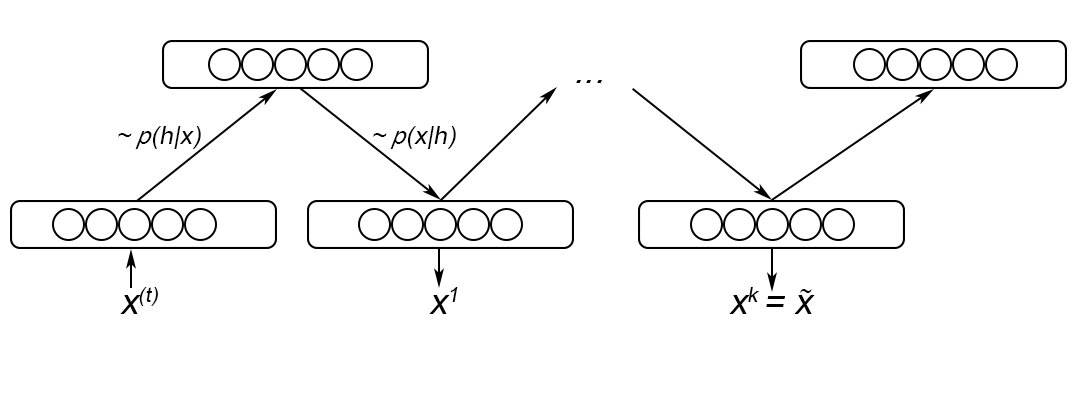
\includegraphics[width=120mm, keepaspectratio]{figures/gibbs}
\caption{A gibbs mintav�telez�si elj�r�s. Forr�s: \protect\url{http://recognize-speech.com/images/nicolas/Gibbs.png}} 
\label{fig:gibbs}
\end{figure}

Ahol $\mathcal{c}$ �s $\mathcal(b)$ az eltol�s s�lyvektorokat jelzik.

\paragraph{Az RBM �s DBN el�tanul�s eredm�nyei} Az hogy a h�l�t el�tan�tjuk fantasztikus eredm�nyjavul�st hozott, amely beigazolta hogy val�ban a sz�mok val�s jellemz� reprezent�ci�ihoz k�zel helyezkedik el egy nagyon optim�lis lok�lis minimum. Az \tabref{MlpEloTablazat}~t�bl�zat szeml�lteti az eredm�nyeit az MNIST adathalmazon. L�tszik hogy ennek seg�ts�g�vel j�val nagyobb h�l�k k�pezhet�ek ki �s l�nyeges jobb eredm�nyre vezetnek.

\begin{table}[ht]
	\footnotesize
	\centering
	\caption{Az MLP teljes�tm�nye az MNIST adathalmazon} \label{tab:MlpEloTablazat}
	\begin{tabular}{ | l | c | c |}
	\hline
	R�tegek sz�ma & neuron strukt�ra & Teszt szet hiba sz�zal�k \\ \hline
	3-r�teg & 768-800-10 & 0.7 \\
	6-r�teg & 784-2500-2000-1500-1000-500-10 & 0.35 \\
	\hline
	\end{tabular}
\end{table}

\subsection{State of the art MLP h�l�zatok}
\paragraph{Tov�bbi kutat�sok} Az MLP h�l�zatokat a mai napig nagy �rdekl�d�s �vezi egyszer� strukt�r�juk miatt. L�tszik hogy az MNIST adathalmazon m�r nem nagyon van hova jav�tani az MLP-k teljes�tm�ny�t, viszony mint azt p�r paragrafussal el�bb megeml�tettem a param�ter t�r cs�kkent�s�ben m�g van fejleszteni val� ezeken a strukt�r�kon. Egy igen friss publik�ci� amelynek c�me "How far can we go without convolution: Improving fully-connected networks"\cite{mlpFrontier} arra mutat r� hogy hogyan lehet az MLP h�l�zatok param�ter ter�t �gy cs�kkenteni hogy a sigmoid r�tegek k�z� kis m�ret� line�ris r�tegeket tesz�nk be, p�ld�nak ok��rt legyen a k�t r�teg 1500-2000 neuron, akkor a teljes param�ter ter�k $1500 * 2000 = 3 000 000$, de ha k�z� tesz�nk egy 500 neuronos line�ris r�tege, akkor ez lecs�kken $150 * 500 + 2000 * 500 = 1 075 000$ param�terre, ami igen szignifik�ns redukci�t jelent a h�l�zat komplex�t�s�ban. Ez a redukci� oly m�rt�k� hogy a fentebb eml�tett publik�ci�ban vizsg�lt legnagyobb strukt�ra param�ter ter�g 112 milli�r�l 2.5 milli�ra cs�kkentett�k, �sszehasonl�t�s k�ppen egy modern konvoluci�s h�l�nak 3.5 milli� param�tere van. L�that� hogy ezzel siker�lt a kutat�knak megoldania a t�bbr�teg� perceptron g�pek egyik legnagyobb probl�m�j�t, a m�rt�ktelen�l burj�nz� param�ter teret. Ezen fel�l az elt�n� gradiensek probl�m�j�t is orvosolja, amivel itt b�vebben nem foglalkozunk. Viszont az eredm�nyeit a CIFAR-10 \figref{mlpEvolution}~�bra szeml�lteti. Az el�bb eml�tett t�bl�zat nagyon j�l �sszefoglalja az MLP-k teljes�tm�ny�nek a fejl�d�s�t a CIFAR-10es adathalmazt haszn�lva.

\begin{figure}[!ht]
\centering
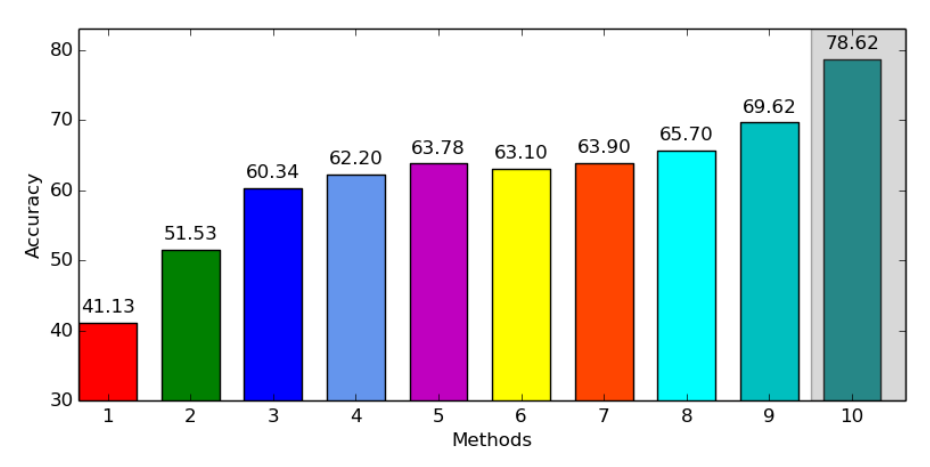
\includegraphics[width=120mm, keepaspectratio]{figures/mlpEvolution}
\caption{Az MLP fejl�d�se a CIFAR-10 adahalmazon. (1) Logiszikus regresszi� feh�r�tett adatokon; (2) Tiszta backpropagation egy 782-10000-10 m�ret� h�l�zaton; (3)  Tiszta backpropagation egy 782-10000-10000-10 m�ret� h�l�zaton. (4) Egy 10000-10000-10es h�l�zaton, RBM el�tan�t�ssal, az utols� r�teg logisztikus regresszi�; (5) Egyr�teg� 10000 neuronos h�l�zat logisztikus regresszi�s kimenettel, RBM el�tan�t�ssal; (6) "Fastfood FFT" model (7) Zerobias autoencoder h�l�zat 4000 rejtett neuronnal �s logisztikus regresszi�s kimenettel; (8) 782-4000-1000-4000-10 Z-Lin h�l�zat; (9) 782-4000-1000-4000-1000-4000-1000-4000-10 Z-Lin h�l�zat dropoutokkal; (10) Ugyanaz mint a (8), csak adat augment�ci�val. Az (1)-(5) eredm�nyek Krizhevsky �s Hinton 2009-es publik�ci�j�b�l sz�rmaznak. A legutols� az�rt sz�rk�tett, mert adat augment�ci�t haszn�l.} 
\label{fig:mlpEvolution}
\end{figure}


\subsection{Konvoluci�s h�l�zatok}
% TODO: Cat's visual cortex p�rhuzam
\paragraph{Bevezet�s} A szakdolgozatom harmadik nagy r�sz�t a konvoluci�s h�l�zatok teszik ki. Miut�n az irodalomkutat�som k�zben r� kellett j�nn�m hogy az �ltalam tanult klasszikus MLP strukt�r�k nem k�pesek a komplex jelek, mint p�ld��l az MNIST adathalmazn�l �sszetettebb k�pek kiel�g�t� megtanul�s�ra, k�nytelen voltam �j ir�nyok ut�n n�zni. �gy tal�ltam meg a konvoluci�s architekt�r�kat. Ezek korunk legjobban teljes�t� architekt�r�i, ennek oka hogy a jelek nagy r�sze amit fel szeretn�nk dolgozni az emberi �rz�kszervek �ltal �rz�kelt jelek, p�ld��l k�pek. Ezek viszont jelent�s transzl�ci�s invarianci�val rendelkeznek, �s ha ezt az invarianci�t nem kell megtanulni hanem bele tudjuk �p�teni a h�l�zat strukt�r�j�ba, akkor l�nyegesen kevesebb param�tert kell megtanulnunk mint egy \emph{elm�leti s�kon} hasonl� teljes�tm�ny� MLP-n�l. Mivel term�szetesen tudjuk Cybenko (1989)\cite{cybenko} �s Kurt Hornik (1991)\cite{hornik} publik�ci�i ut�n hogy egy k�tr�teg� MLP-vel tetsz�leges f�ggv�nyt k�pes approxim�lni, de ehhez annyi neuron kellene a komplex jelek eset�ben mint a k�pek hogy praktikusan nem kivitelezhet�ek ezek a h�l�zatok. A r�tegek n�vel�s�vel �s h�l�zati k�nyszerek bevezet�s�vel ez a param�ter t�r jelent�sen cs�kkenthet�.

\paragraph{Az intuici�} A konvoluci�s architekt�ra teljes m�rt�kben biol�giailag inspir�lt, a macsak vizu�lis kortex�nek a felt�rk�pez�s�n�l tal�ltak hasonl� kapcsolatokat az �llat agy�ban, �s ennek a mint�j�ra �p�tett�k fel a mesters�ges h�l�zatot. Alap�tlete hogy mag�ba a h�l�zati strukt�r�ba foglaljuk bele a jel transzl�ci�s invarianci�j�t. A modellt eleinte k�pek feldolgoz�s�ra alkott�k meg, �s az el�bbi mondat itt is szeml�ltethet� a legintuitivabban. Tegy�k fel hogy van egy k�p�nk amin vagy egy objektum, akkor ha fel kell ismerni hogy a k�p az adott objektumnak a jellemz�it tartalmazza-e akkor nek�nk adott esetben ugyan annyi inform�ci�val szolg�l ha ez a jellemz� (mondjuk egy sarok) a bal vagy a jobb oldalon van a k�pen. Term�szetesen ezek a lok�lis strukt�r�k a r�tegekkel felfele egyre glob�lisabbak lesznek, az egyre magasabb szinteken pedig t�bb jellemz�b�l kompon�lt �ssztetett jellemz�k jelennek meg. �s a h�l�zat az �sszetett jellemz�k jelenl�t�b�l k�vetkeztet a k�p oszt�ly�ra. Ezt hivatott szeml�ltetni a \figref{deconvnet}~�bra �s \figref{deconvnet2}~�bra amely egy konvoluci�s h�l� egyes r�tegeinek a sz�r�it mutatja be, �s hogy milyen k�pelemek aktiv�lt�k �ket a legink�bb. Az els� sikeres alkalmaz�sa ennek a modellnek a LeNet\cite{leNet} volt 1990-ben, amelyet ir�ny�t�sz�mok, karakterek �s hasonl� dolgok felismer�s�re haszn�ltak, de a modell sok�ig nem kapott nagy �rdekl�d�st.

\begin{figure}[!ht]
\centering
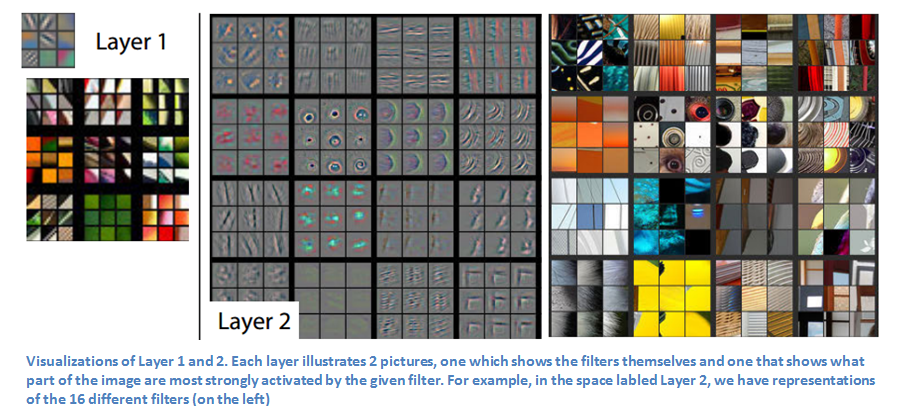
\includegraphics[width=120mm, keepaspectratio]{figures/deconvnet}
\caption{Az els� k�t szint sz�r�i egy konvoluci�s h�lozatban. Forr�s: "Visualizing and Understanding Convolutional Neural Networks" \cite{deconvnet}} 
\label{fig:deconvnet}
\end{figure}

\begin{figure}[!ht]
\centering
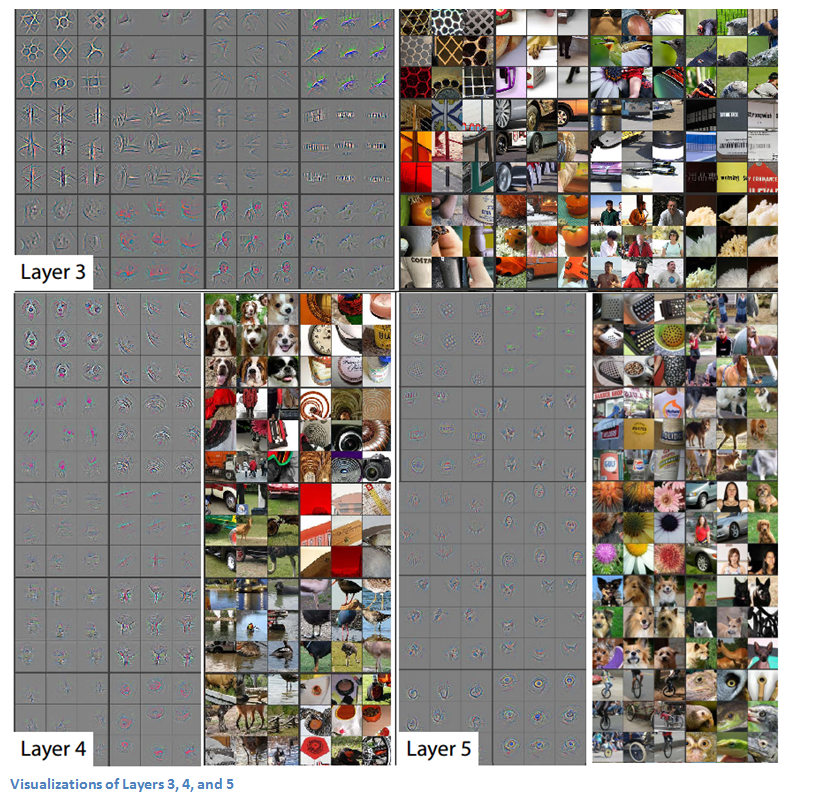
\includegraphics[width=120mm, keepaspectratio]{figures/deconvnet2}
\caption{Az fels�bb r�tegek sz�r�i egy konvoluci�s h�lozatban. Forr�s: "Visualizing and Understanding Convolutional Neural Networks" \cite{deconvnet}} 
\label{fig:deconvnet2}
\end{figure}

\paragraph{Matematikai interpret�ci�ja} Tegy�k fel hogy van egy $32x32x3$-as k�p�nk. Ahhoz hogy egy teljes r�tegbe kapcsoljuk bele mondjuk $1024$ neuronnal ki kellene lap�tanunk, �s egy $32 * 32 * 3 * 1024 = 3'145'728$ param�ter�nk lenne az els� r�tegben. De tegy�k fel hogy a legkissebb jellemz� amit �rz�kelni akarunk az egy $3x3$ m�ret� patchen van a k�pen, viszont ak�rhol lehet, akkor ha az els� r�tegben $32$ jellemz�t szeretn�nk �rz�kelni, akkor csak $3 * 3 * 32 = 288$ param�terre lesz sz�ks�g�nk az els� r�tegben, ami jelent�s redukci�. Ezut�n a k�vetkez� r�teg ehhez a $288$ neuronhoz fog kapcsol�dni, �s ha ott 64 neuron lesz akkor $3*3*64 = 567$ neuronra kell majd, amik az eredeti k�pb�l viszont m�r egy $5x5$-�s szeletet fognak indirekt m�don lefedni. Ezt mutatja be egy klasszikus architekt�ra a leNet a \figref{leNet}~�br�n.

\begin{figure}[!ht]
\centering
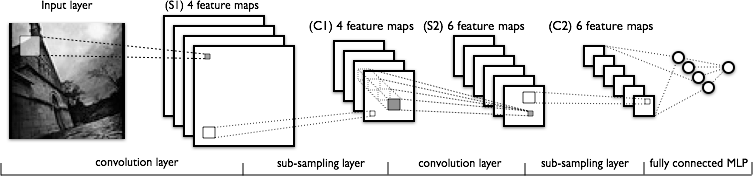
\includegraphics[width=120mm, keepaspectratio]{figures/leNet}
\caption{Az fels�bb r�tegek sz�r�i egy konvoluci�s h�lozatban. Forr�s: "Visualizing and Understanding Convolutional Neural Networks" \cite{deconvnet}} 
\label{fig:leNet}
\end{figure}
\paragraph{Az IMAGNET} 2012-ben az AlexNet nev� konvoluci�s h�l�zat amelyet Alex Krizhevsky, Ilya Sutskever �s Geoffrey Hinton alkottak f�l�nyesen megnyerte az az�vi ILSVRC versenyt. A h�l� top 5 hib�ja (az olvas� konzult�ljon az adathalmazokat bemutat� r�sszel a metrika le�r�s��rt.) 16\% volt, m�g a m�sodik helyete ami egy SVM-eket haszn�l� modell volt 26\%-os hib�t produk�lt. Ez a 10\%-os k�l�ns�g az egekbe emelte a konvoluci�s h�l�zatok n�pszer�s�g�t, �s hivatalosan is elhozta a neur�lis k�pfeldolgoz�s kor�t. Innent�l kezdve minden �vben konvoluci�s h�l�zatok nyert�k meg az ILSVRC-t. A \tabref{ImagenetTable}~t�bl�zat bemutatja az egyes �vek eredm�nyeit a h�l�t n�h�ny param�ter�vel egy�tt. �sszehasonl�t�s k�ppen, egy �tlagos ember teljes�tm�nye az adathalmazon 5-10 hibasz�zal�k k�r�l mozog. 

\begin{table}[ht]
	\footnotesize
	\centering
	\caption{Az ILSVRC gy�ztesei} \label{tab:ImagenetTable}
	\begin{tabular}{ | c | c | p{5cm} | c | c |}
	\hline
	�v & A strukt�ra neve & Tan�t�s ideje & Param�ter t�r m�rete & Top 5 hiba sz�zal�k \\ \hline
	2012 & AlexNet \cite{alexNet} & k�t GTX 580 GPU-n 5-6 nap & 60 milli� & 16\% \\
	2013 & ZF Net \cite{deconvnet} & egy GTX 580 GPU-n 12 nap & ~60 milli� & 11.2\% \\
	2014 & GoogLeNet \cite{googLeNet} & "n�h�ny high end GPU-n egy h�ten bel�l" & 4 milli� & 6.7\% \\ 
	2015 & Microsoft ResNet \cite{resNet} & 8 GPU-s g�pen 2-3 h�tig & N\textbackslash A & 3.6\% \\
	\hline
	\end{tabular}
\end{table}

\paragraph{�rt�kel�s} L�that� hogy a leg�jabb konvoluci�s architekt�r�k m�r az emberi ki�rt�kel�sn�l is pontosabb eredm�nyt hoznak. R�ad�sul a kezdeti na�v megk�zel�t�st k�vet�en a param�ter t�r is drasztikus cs�kken�snek indult. Manaps�g ha valaki k�poszt�lyoz�si feladatot szeretne v�gezni neur�lis h�l�zatokkal, akkor egy ilyen el�re elk�sz�tett architekt�r�t fog haszn�lni. Sajnos az is j�l nyomonk�vethet� hogy a h�l�zatok fejl�d�s�vel a sz�ks�ges hardware kapacit�s is meredek emelked�snek indult. Ha az ember egy konvoluci�s architekt�r�t egy saj�t adathalmazra szeretne megtan�tani akkor komoly infrastrukt�r�val kell rendelkeznie hozz�. �ppen itt domborodik ki a tensorflownak a dolgozat elej�n eml�tett el�nye, hogy miut�n pythonban specifik�ltuk a strukt�r�t azt k�pesek vagyunk minden er�fesz�t�s n�lk�l egy 8 GPU-s f�rtre sz�tterjeszteni �s tan�tani, majd ut�na a param�ter teret lementve ak�r egy mobilon a megtan�tott h�l�t �jra bet�lteni �s ak�r val�s idej� inferenci�t futtatni. A param�ter t�r ha 16 bites floatokkal sz�mol az ember akkor 4 milli� param�tern�l kb 8 megabyte lesz, ami m�g egy igen kezelhet� mennyis�g.

\section{Tov�bbi �rdekes ir�nyok a neur�lis k�pfeldolgoz�sban}

Itt, az irodalom kutat�som t�rgyal�s�nak v�g�n el�rt�nk arra a pontra ahol �ppen a tudom�ny tart, ebben a fejezetben r�viden fel szeretn�m villantani a neur�lis k�pfeldolgoz�s leg�jabb �s leg�rdekesebb ir�nyait. 

\paragraph{R�gi� alap� konvoluci�s h�l�zatok\cite{rcnn}} Sokan azt mondj�k hogy ez a publik�ci� csokor (R-CNN, Fast R-CNN, Faster R-CNN) hossz� id�k �ta az egyik legfontosabb amit �j neur�lis architekt�r�kr�l olvashatott az ember. Eddig meg tudtuk mondani egy h�l�val hogy tartalmaz-e a k�p valamilyen objektumot. Az R-CNN h�l�zatok m�r az objektum pontos hely�t is megmondj�k a k�pen, ami egy min�s�gbeli ugr�st jelent. Az \figref{FasterRCNN}~�bra szeml�lteti a m�dszert. A m�dszer l�nyege hogy a feladat k�t neur�lis h�l�zatra van faktoriz�lva amik tandemben dolgoznak, az egyik egy oszt�ly agnosztikus objektum detektor, m�g a m�sik egy oszt�lyoz� h�l�zat.

\begin{figure}[!ht]
\centering
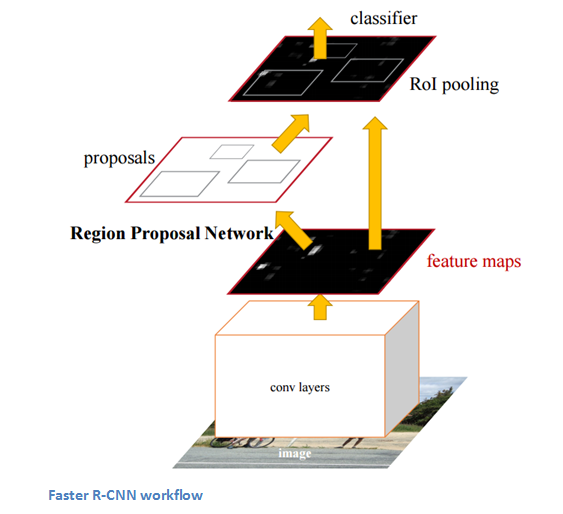
\includegraphics[width=70mm, keepaspectratio]{figures/FasterRCNN}
\caption{A Faster R-CNN munkafolyamata} 
\label{fig:FasterRCNN}
\end{figure}

\paragraph{Generat�v adverzi�lis h�l�zatok\cite{genAdvNet}} A LeCunn, a konvoluci�s h�l�k megalkot�ja szerint ez az ut�bbi 10 �v leg�rdekesebb �tlete a ter�leten. A l�nyeg hogy k�t h�l�zatot tan�tunk tandemben, egy generat�v �s egy diszkriminat�v modell-t. A diszkriminat�v modell dolga ed�nteni egy k�pr�l hogy val�di-e vagy sem, a generat�v� pedig hogy olyan k�peket tudjon gener�lni amivel �tveri a m�sik modell-t, ez�rt h�vj�k adverzi�lis h�lozatnak. Az eg�sz s�lya abban rejlik hogy �gy a diszkriminat�v h�l�zatnak meg kell tanulni az adat egy nagyon j� reprezent�ci�j�t hogy k�pes legyen d�nteni, ezzel mintegy nem fel�gyelt m�don a legfontosabb jellemz�ket kiemelni a k�pb�l. A gener�tor a v�g�re pedig k�pes lesz val�s�gh� k�peket "�lmodni". A figref{adversarial}-�bra mutat egy tipikus tan�t� p�ld�t.

\begin{figure}[!ht]
\centering
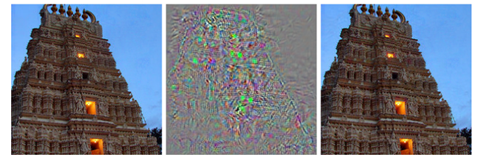
\includegraphics[width=70mm, keepaspectratio]{figures/adversarial}
\caption{Jobbra: Eredeti k�p, k�z�pen: Pertub�ci�k, balra: Pertub�lt k�p. A jobb oldalit helyesen, a bal-t pedig hib�san oszt�lyozn� egy CNN.} 
\label{fig:adversarial}
\end{figure}

\paragraph{K�ple�r�sok gener�l�sa\cite{genImgDesc}} A nem olyan t�voli m�ltban nagyon sok �rdekes publik�ci� jelent meg olyan neur�lis strukt�r�kr�l amelyek k�pek le�r�s�ra alkalmasak. L�nyeg�ben egy CNN �s egy RNN h�l�zat m�k�dik egy�tt, �s fantasztikus dolgokra k�pesek. Tov�bb nem is taglaln�m, mert nagyon sok el�ismeretet ig�nyel a t�ma, az �rdekl�d�k a megfelel� publik�ci�t megtal�lj�k az irodalomjegyz�kben \cite{generatingImageDesc}. A \figref{generatingImageDesc} mutatja az eredm�nyt.

\begin{figure}[!ht]
\centering
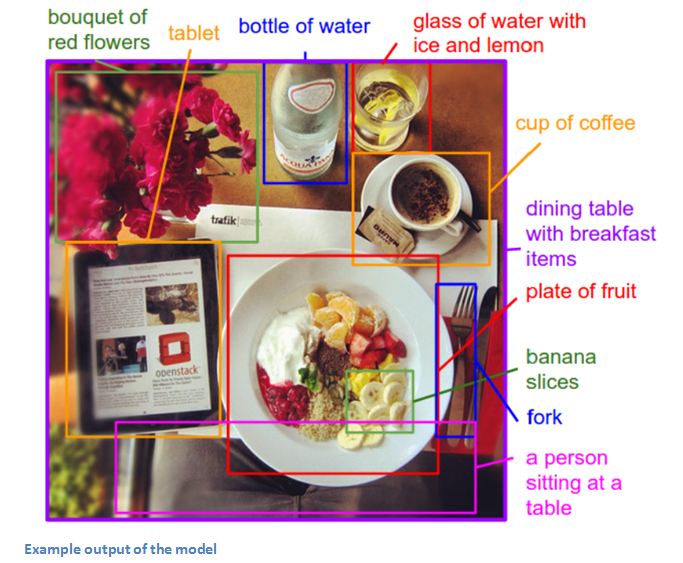
\includegraphics[width=70mm, keepaspectratio]{figures/caption}
\caption{A Faster R-CNN munkafolyamata} 
\label{fig:generatingImageDesc}
\end{figure}

\paragraph{T�rbeli transzform�ci�s h�l�zatok (STN \cite{stn})} A fejleszt�s jelent�s�ge abban rejlik hogy eddig mindig vagy a h�l� strukt�r�j�ba kellett belek�dolni ha valamilyen variancia ellen v�deni szerett�k volna a h�l�zatot, vagy pedig az adathalmazt kellett �gy augment�lni hogy a h�l� j�l �ltal�nos�tson. Az el�bbire egy j� p�lda a CNN h�l�zatok max-pooling r�tege, az ut�bbira pedig az hogy mondjuk minden k�pet elforgatva is beadunk a h�l� tan�t�sakor, hogy invari�ns legyen rot�ci�ra a megtanult modell. Az STN h�l�zatok mint egy modulk�nt kapcsolhat�ak az egyes h�l�zatok el�, �s ezeket a probl�m�kat megfelel� tan�t�s ut�n automatikusan megoldj�k. J�l l�that� hogy a neur�lis fejleszt�s a monolitikus h�l�zatokb�l szint�n elkezdett a modulokb�l fel�p�l� paradigma fel� menni. Az \figref{STN}~�bra mutat a h�l�zat m�k�d�s�re egy p�ld�t.

\begin{figure}[!ht]
\centering
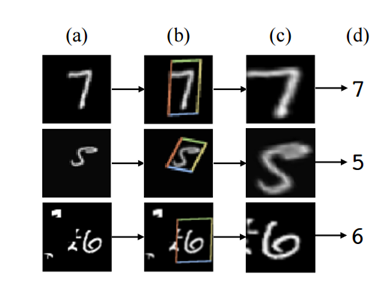
\includegraphics[width=70mm, keepaspectratio]{figures/stn}
\caption{Egy t�rbeli transzform�ci�s h�l�zat l�p�sei.} 
\label{fig:STN}
\end{figure}

%----------------------------------------------------------------------------
\chapter{H�l�zatok impelment�l�sa �s elemz�se tensorflowban}
%----------------------------------------------------------------------------

A k�vetkez� r�szben szeretn�m bemutatni saj�t muk�mat �s m�r�si eredm�nyeimet. Az el�z� r�szben bemutatott h�l�zatfajt�kb�l megval�s�tottam sz�mtalan p�ld�nyt tensorflowban, �s m�r�seket v�geztem rajtuk az MNIST �s a CIFAR-10 adathalmazon. A munk�m c�lja az volt hogy leteszteljem a tensorflow lehet�s�geit k�s�rleti h�l�zatok kifejleszt�s�re �s monitoroz�s�ra. A fejezet a k�vetkez� r�szekre tagolhat�:
\begin{enumerate}
\item A baseline met�dusok bemutat�sa.
\item A fejleszt�si k�rnyezet bemutat�sa.
\end{enumerate}

\section{A baseline oszt�lyoz�k}
Term�szetesen nem lehet m�r�seket v�gezni baselineok n�lk�l, ez�rt a CIFAR-10 �s az MNIST adathalmazon is lefuttattam k�t ismert, minden neh�zs�g n�lk�l haszn�lhat� oszt�lyoz� algoritmust. Az egyik a Logisztikus regresszi� volt, a m�sik pedig az SVM. Mindkett� bemenet�re k�zvetlen a k�p pixeljeit tettem.

\section{A saj�t magam �ltal kialak�tott fejleszt�k�rnyezet}
A Tensorflow �kosziszt�ma nagyon j� pontja a cs�csra j�ratott monitoroz�si lehet�s�gek, viszont nem trivi�lis egy olyan strukt�ra kialak�t�sa ahol az ember nagy hat�konys�ggal dolgozhat. Hosszas k�s�rletez�s ut�n a k�vetkez� munkafolyamatot tal�ltam a legjobbnak:
\begin{itemize}
\item \emph{Gyors prototipiz�l�s:} Erre a c�lra a Jupyter notebookokba �rt TF-Slim magas szint� API-t tal�ltam a legjobbnak, �gy nagyon gyorsan le lehet ak�rmilyen �tletet tesztelni �s ki�rt�kelni.
\item \emph{Stabil modellek fejleszt�se:} Ha egy modell t�ljutott a p�r soros m�reten, vagy t�nyleg egy nagyobb rendszer r�szek�nt szeretn�nk haszn�lni akkor azt �rdemesnek tal�ltam oszt�lyba foglalni, �s a fejleszt�shez PyCharm IDE-t haszn�lni mert l�nyegesen gyorsabban lehet vele haladni komplex python k�dn�l mint a notebookokkal. 
\item \emph{A modellek ki�rt�kel�se:} A modellek ki�rt�kel�s�re �gy gondolom hogy a Tensorflowval �rkez� Tensorboard a legalkalmasabb, mint majd l�tni fogja az olvas� a modelleim elemz�s�n�l hogy ez az eszk�z lehet�v� teszi komplex strukt�r�k elemz�s�t eg�szen a tanul�st�l az ig�nyelt rendszer er�forr�sokig.
\item \emph{A modellb�l kinyert adatok r�szletes elemz�se:} Erre a c�lra az klasszikus tudom�nyos csomagok haszn�lat�t tal�ltam a legjobbnak jupyter notebookban alkalmazva, mert �gy egy helyen van a modell futtat�sa, a m�r�si eredm�nyek �s azt elemz� k�d.
\item \emph{Egzotikusabb modellek kivitelez�se:} Ha az ember olyan modelleket szeretne k�dolni amik t�lny�lnak a klasszikus el�recsatolt strukt�r�kon akkor k�nytelen leny�lni a Tensorflow eredeti programoz�si absztrakci�j�hoz, mint ahogyan azt az RBM eset�ben l�tni fogjuk. Ez az alacsony API hatalmas szabads�got ad a programoz�nak, de iszonyatosan b�szav� (verbose).
\end{itemize}

\section{A saj�t implement�ci�k bemutat�sa}
\subsection{A h�l�zatok monitoroz�sa}
A Tensorflow kifejlett API-t k�n�l a h�l�zat param�tereinek k�vet�s�re tanul�s k�zben, de nem ment le automatikusan minden egyes lefut�skor minden v�ltoz� �rt�k�t, mivel ez egy modern h�l�zatn�l t�bb milli� �rt�ket is jelenthet. A VGG konvoluci�s h�l� p�ld�ul 140 milli� param�tert tartalmaz. A h�l�zatr�l �ltal�noss�gban a k�vetkez� �rt�keket mentettem le: minimum �rt�k, maximum �rt�k, k�z�p �rt�k �s a standardiz�lt sz�r�sukat. hogy ezeket ne kelljen minden v�ltoz�ra kiadni, ez�rt a \listref{variableSummaries}-es f�ggv�nyt alkalmaztam.

\begin{lstlisting}[frame=single,float=!ht,caption= A v�ltoz�k ment�se label=listing:variableSummaries, mathescape=true]
def variable_summaries(name, var):
    """Attach a lot of summaries to a Tensor."""
    with tf.name_scope('summaries'):
        mean = tf.reduce_mean(var)
        tf.scalar_summary('mean/' + name, mean)
        with tf.name_scope('stddev'):
            stddev = tf.sqrt(tf.reduce_sum(tf.square(var - mean)))
        tf.scalar_summary('sttdev/' + name, stddev)
        tf.scalar_summary('max/' + name, tf.reduce_max(var))
        tf.scalar_summary('min/' + name, tf.reduce_min(var))
        tf.histogram_summary(name, var)
\end{lstlisting}

\subsection{A logiszikus regresszi�}
Az els� modell amit implement�ltam Tensorflowban az a logisztikus regresszi� volt. A c�lja az volt hogy �sszehasonl�tsam a Tensorflow er�forr�s ig�ny�t egy klasszikus python machine learning csomag, a Scikit-learn ig�nyeivel. A strukt�r�t az <sz�m>~�bra szeml�lteti. Egyb�l l�tsz�dhat hogy az avatatlan szem sz�m�ra a tensorboard el�gg� nehezen �rtelmezhet� lehet, ez�rt is szokt�k mondani hogy a tensorflownak a tanul�si g�rb�je viszonylag nagy. Szerencse hogy lehet benne n�vtereket l�trehozni hogy a gr�fok k�nnyebben �tl�that�ak legyenek. Az eg�sz tanul�si gr�fot a j�rul�kos nodeokkal az <sz�m>~�bra szeml�lteti.

\subsection{A t�bbr�teg� perceptron}
A t�bbr�teg� perceptronnal val� k�s�rletez�st a TF-Slim API nagyon megk�nny�ti, minden neh�zs�g n�lk�l a r�tegeket egym�s ut�n tenni, ha pedig egyedi elemet szeretne az ember defini�lni akkor arra is lehet�s�g van. Hasonl� architekt�r�kat teszteltem az MNIST �s a CIFAR-10 adathalmazon is, ami nagyon j�l megfogta a k�t adathalmaz k�z�tti k�l�nbs�get. A \listref{MlpDef}-list�z�s egy ilyen h�l� definici�j�t szeml�lteti.

\begin{lstlisting}[frame=single,float=!ht,caption= Egy MLP definici�ja, label=listing:MlpDef, mathescape=true]
def fully_connected(batch_data, batch_labels):
    with slim.arg_scope([slim.fully_connected],
                      activation_fn=tf.nn.relu,
                      weights_initializer=tf.truncated_normal_initializer(0.0, 0.01),
                      weights_regularizer=slim.l2_regularizer(0.0005)):
        # First Layer
        x = slim.fully_connected(batch_data, 400, scope='fc/fc_1')
        variable_summaries('fc/fc_1', x)
        
        # Second Layer
        x = slim.fully_connected(x, 1024, scope='fc/fc_2')
        variable_summaries('fc/fc_2', x)
        
        # Third Layer
        last_layer = slim.fully_connected(x, 10, activation_fn=None, scope='fc/fc_3')
        variable_summaries('fc/fc_3', x)
        predictions = tf.nn.softmax(x)
 
    	slim.losses.softmax_cross_entropy(last_layer, batch_labels)
	    total_loss = slim.losses.get_total_loss()
   	 	tf.scalar_summary('losses/total_loss', total_loss)
    
    	optimizer = tf.train.GradientDescentOptimizer(learning_rate=0.01)
        return optimizer, predictions
\end{lstlisting}

Mint l�that� nagyon k�nnyen �ll�that�ak a reguraliz�ci�s tagok, megadhat� t�bb f�let optimaliz�l� �s hibaf�ggv�ny is, ami igaz�n k�nny�v� tette a k�s�rletez�st.

\subsection{Az RBM h�l�zat}
Mint mondtam a TF-Slim nagyon k�nyelmes volt addig am�g olyan strukt�r�kkal dolgoztam amik k�nnyen defini�lhat�ak. Viszont csak t�bbr�teg� perceptronok �s konvoluci�s h�l�zatokat lehet benne egyel�re alkotni. Az korl�tozott boltzmann g�p implement�l�s�hoz le kellett mennem a Tensorflow alacsony szint� interfac�hez amiben a h�l�zat implement�l�sa t�bb mint egy h�t volt. Viszont ezalatt �rtettem meg igaz�n hogy hogyan m�k�dik egyr�szt a k�nyvt�r, m�sr�szt pedig az RBM-ek. 
Az RBM strukt�ra legtr�kk�sebb r�sze a kontraszt�v divergencia volt, mivel az egy val�sz�n�s�gi d�nt�s, de az egyes batchek fut�sa k�zben nem tudok k�zvetlen�l a gr�fon bel�l v�letlen sz�mokat gener�lni v�ltoztathat� mennyis�gben. Az�rt nem lehet egy adott m�retben gener�lni, mert a batch m�ret v�ltozik, �s minden sz�mnak kellett gener�lni.
A megold�s amit alkalmaztam az az volt hogy numpy-ban legener�ltam minden tan�t�sn�l egy akkora m�trixot v�letlen sz�mokb�l mint amekkora a tan�t� halmazom volt. Majd a bin�ris 0-1 d�nt�st a k�vetkez� k�ppen szimul�ltam:
\begin{enumerate}
\item Kivontam a val�szin�s�gi m�trixot a random sz�mokb�l
\item Vettem az elj�jel�t a keletkezett m�trixnak
\item �tvezettem egy relu r�tegen, amit�l 0 �s 1 k�z� normaliz�l�dott.
\end{enumerate}

\paragraph{A tan�t�s} A tan�t�st k�tf�le k�ppen v�geztem el, egyr�szr�l defini�ltam a szabad energia f�ggv�nyt �s a keretrendszerrel sz�moltattam ki a \eqref{rbmPFromEnergy} f�ggv�nyb�l �s k�l�nb�z� be�p�tett optimaliz�torokkal teszteltem, gradientdescenttel �s Adamsoptimizerrel. Illetve a k�s�rletez�s egy m�sik dimenzi�ja az volt hogy egyes esetekben megengedtem az RBM fel� kapcsolt regresszornak hogy az el�re megtanult s�lyokat v�ltoztassa (ezt h�vjuk fine-tuning-nak), m�s esetben pedig nem. M�sr�szt k�zvetlen kisz�moltam a gibbs sampling ut�ni �rt�kekb�l \eqref{RbmWDirect}, \eqref{RbmCDirect} �s \eqref{RbmBDirect} f�ggv�nyeket �s egyszer�en csak hozz�adtam �ket a s�lyvektorhoz. A \figref{RbmClosed}~�bra a h�l�zat mad�rt�vlati strukt�r�j�t szeml�lteti. K�nnyen kivehet� hogy egy softmax r�teg is hozz� van csatolva az RBM magj�hoz, miut�n fel�gyelet n�lk�l tan�tom az RBM-et az a r�teg v�gzi az oszt�lyz�st. A \figref{rbmExpanded}~�bra pedig az RBM bels� strukturj�t mutatja. Itt l�tszik igaz�n hogy a Tensorboard grafikonjai milyen kifonomult vizualiz�ci�t tesznek lehet�v�. A tan�t�s optimaliz�l�s�t a \cite{rbmGuide} alapj�n v�geztem.

\begin{figure}[!ht]
\centering
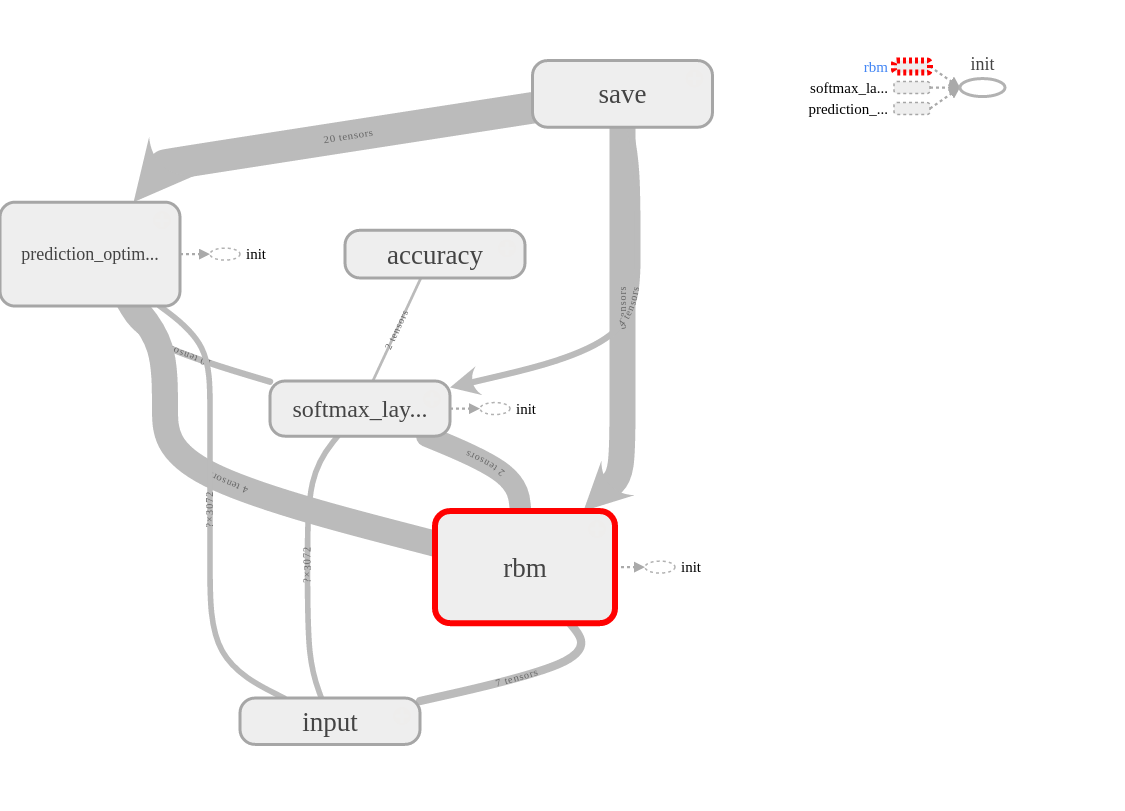
\includegraphics[width=100mm, keepaspectratio]{figures/rbmClosed}
\caption{} 
\label{fig:rbmClosed}
\end{figure}

\begin{figure}[!ht]
\centering
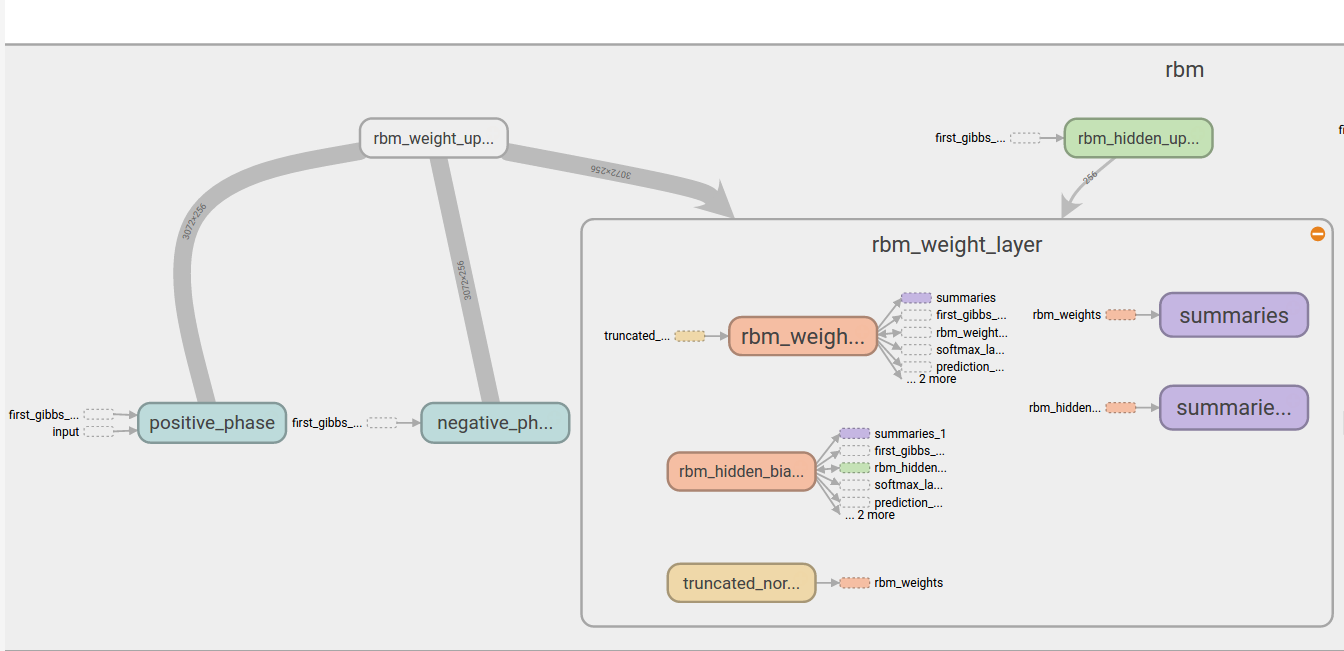
\includegraphics[width=100mm, keepaspectratio]{figures/rbmExpanded}
\caption{} 
\label{fig:rbmExpanded}
\end{figure}

\subsection{Hibrid modellek}
A k�s�rletez�s�nk sor�n elkezdt�nk olyan architekt�r�kkal foglalkozni ahol a kimenet nem a neur�lis h�l�zat r�sze, mint p�ld�ul az RBM oszt�lyoz�k �ltalam tesztelt vari�ns�n�l, hanem a kimeneti aktiv�ci�k val�sz�n�s�gi eloszl�s�t adtam be mint�nk�nt egy SVM g�pnek. �gy hatalmas dimenzi� cs�kken�st �rt�nk el, pl 768-r�l 1024-re, ami jelent�sen meggyors�totta az SVM tan�t�s�t, an�lk�l hogy a nyers pixeladatokon tan�tott SVM-hez k�pest romlott volna a modell predikci�s k�pess�ge. Az �ltalam haszn�lt teszt g�pen a CIFAR-10es adathalmaz nyers pixeljeit sajnos nem is tudtam megtan�tani re�lis id� alatt egy SVM-nek.

\subsection{A Konvoluci�s modell}
T�bb konvoluci�s modell-t kipr�b�ltam, a m�r�seim egyik f� ir�nya az volt hogy ugyanazt a modellt prob�lom ki az MNIST �s a CIFAR-10 adathalmazon, �s megn�zni hogy melyik modell hogyan reag�l az adat megn�vekedett komplexit�s�ra. T�bb h�l�zatot kir�b�ltam, az alapmodell fel�p�t�s�t a \figref{convnet_1}~�bra mutatja. A k�s�rleteim arra ir�nyultak hogy plusz teljesen �sszek�t�tt r�tegek hozz�ad�sa, esetleg a konvoluci�s r�tegek m�s elrendez�se milyen eredm�nyre juttat.

\begin{figure}[!ht]
\centering
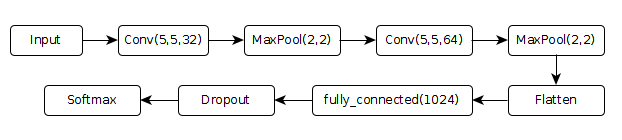
\includegraphics[width=120mm, keepaspectratio]{figures/convnet_1}
\caption{} 
\label{fig:convnet_1}
\end{figure}

\subsection{A konvoluci�s modell sk�l�z�sa}
Az el�bbiekben bemutatott konvoluci�s modell k�nnyed�n tan�that� p�r perc alatt egy korszer� CPU-n, viszont ha az ember nagyobb modelleket szeretne tan�tani akkor ez m�r nem egy re�lis alternat�va. Ezekre az esetekre egy nagyobb h�l�zattal k�s�rleteztem a CIFAR-10 adathalmazon, aminek a fel�p�t�s�te a \figref{convnet_2}~�bra mutatja. 

\begin{figure}[!ht]
\centering
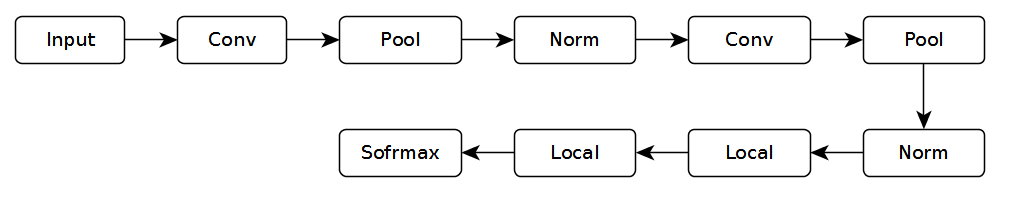
\includegraphics[width=120mm, keepaspectratio]{figures/convnet_2}
\caption{} 
\label{fig:convnet_2}
\end{figure}

Ezt a h�l�zatot teszteltem CPU-n, 1 GPU-n, majd 2 GPU-n. A Tensorflow k�pes a sz�m�t�sokat automatikusan elosztani az eszk�z�k k�z�tt olyan m�don hogy heurisztikusan megkeresi hogy mely oper�ci�k ment�n �rdemes sz�tv�gni a sz�m�t�si gr�fot, majd azokhoz az �lekhez berak k�ld� �s fogad� csom�pontokat, ahogyan a \figref{device_distro}~�bra szeml�lteti.

\begin{figure}[!ht]
\centering
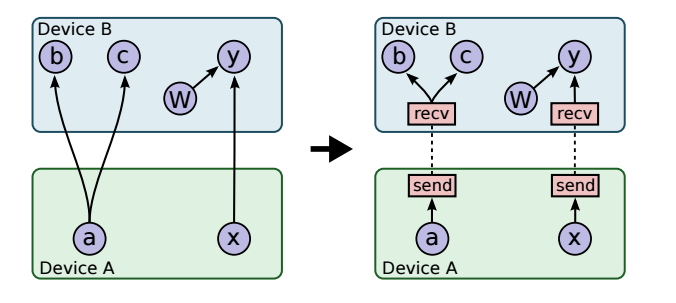
\includegraphics[width=120mm, keepaspectratio]{figures/device_distro}
\caption{} 
\label{fig:device_distro}
\end{figure}

Ez sok esetben teljesen megfelel az elv�r�sainknak, ha nmem szeretn�nk sokat vesz�dni a h�l�zat eloszt�s�val, vagy m�gy is tul nagy a h�l�nk, �s nem f�rne el gradiens sz�m�t�ssal egy�tt rendesen egyetlen eszk�z�n. De ha kissebb a h�l� �s t�bb eszk�z�nk van akkor felmer�lhet a lehet�s�g hogy esetleg jobban meg�rn� a gr�fot egy az egyben lem�solni az egyes eszk�z�kre, �s a s�lyokat a f� mem�ri�ban tartani, majd az egyes p�rhuzamos fut�sok ut�n itt szinkroniz�lni a lefut�sokat. �n ezt a megk�zel�t�st teszteltem le, aminek a neve torony p�rhuzamos tan�t�s, ezt a \figref{tower_parallel}~�bra mutatja.

\begin{figure}[!ht]
\centering
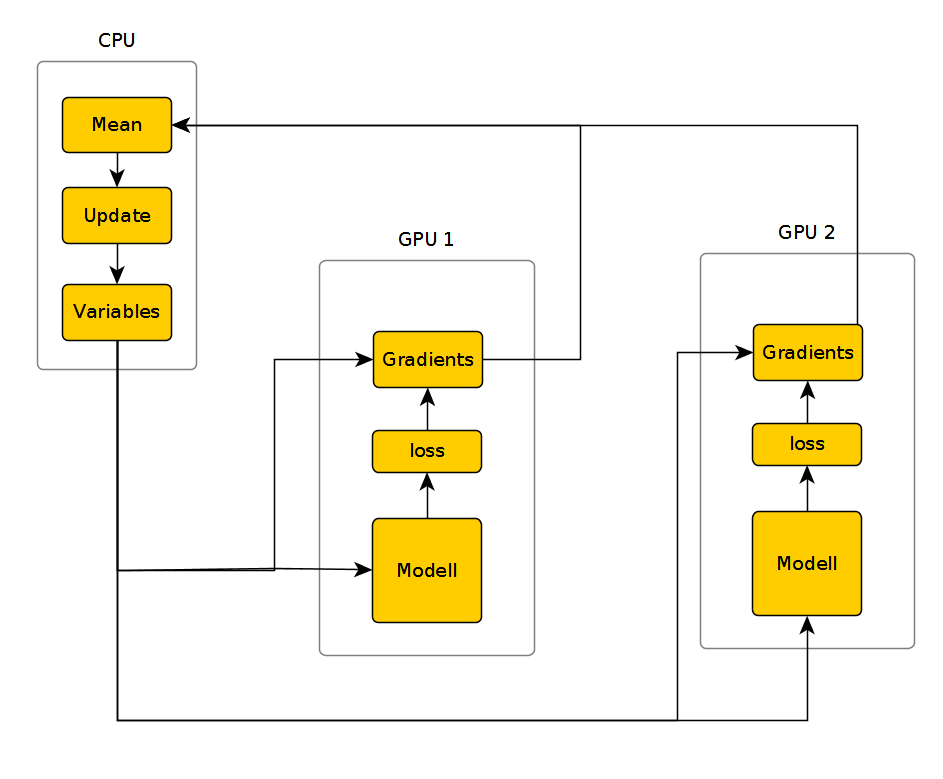
\includegraphics[width=120mm, keepaspectratio]{figures/tower_parallel}
\caption{} 
\label{fig:tower_parallel}
\end{figure}

\chapter{A m�r�si eredm�nyeim �sszegz�se}
Ebben a fejezetben szeretn�m bemutatni az �ltalam elk�sz�tett h�l�zatok fut�s�nak m�r�si eredm�nyeit. �s ezeknek aspektusait:
\begin{enumerate}
\item A keretrendszer �ltal�nos teljes�tm�nye.
\item A baseline eredm�nyek bemutat�sa.
\item Az MLP h�l�zattal el�rt eredm�nyek �s az ezekb�l levont tanuls�gok.
\item A konvoluci�s h�l�zatokkal el�rt eredm�nyek �s ennek �sszegz�se.
\item A hibrid h�l�zatokkal el�rt eredm�nyek.
\end{enumerate}

A g�p specifik�ci� amin �ltal�noss�gban teszteltem (eltekintve a GPU sk�l�z�s r�szt�l) a k�vetkez�ek:
\begin{itemize}
\item Mem�ria: 8 Gigabyte DDR4
\item CPU: Intel Core i7-4702MQ CPU @ 2.20GHz x 8
\end{itemize}
A g�pben elhelyezked� grafikus k�rty�t nem haszn�ltam, az Nvidia hib�s eszk�z meghajt� programja miatt.

\section{A keretrendszer �ltal�nos teljes�tm�nye}
Ebben a r�szben azt vizsg�ltam hogy a tensorflow hogyan b�nik az er�forr�sokkal. Ennek �rdek�ben t�bb dolgot tettem:
\begin{itemize}
\item Egyszer� rendszerszint� m�r�seket futtattam.
\item A Tensorboardon kereszt�l vizsg�ltam a h�l�k teljes�tm�ny �s er�forr�s karakterisztik�j�t.
\item Egy konvoloci�s h�l�t kisk�l�ztam a CPU-r�l 1 GPU-ra, majd 2 GPU-ra.
\end{itemize}

\section{Rendszer szint� m�r�sek.}
Az els� dolog amikor fel�t�tte a fej�t a k�rd�s n�lam, hogy m�gis hogyan viszonyul teljes�tm�nyben a tensorflow a Python de facto g�pi tanul�s eszk�z�hez, a Scikit-learnh�z az volt amikor nem siker�lt lefuttatnom egy logisztikus regresszi�t Scikit seg�ts�g�vel a CIFAR-10 adathalmazon mert a teszt g�p haszn�lhatlann� v�lt. A k�t m�r�s er�forr�s karakterisztik�j�t a \figref{sklearn_cpu}~�bra �s a \figref{tf_cpu}~�bra mutatja, ahol az el�bbi a Scikit-learn az ut�bbi pedig a Tensorflowban megval�s�tott k�zel�t� Logisztikus Regresszi�.

\begin{figure}[!ht]
\centering
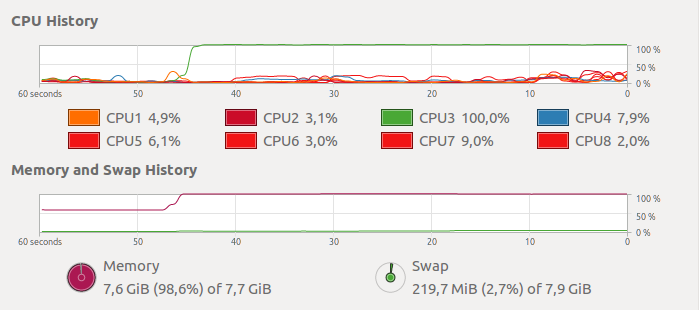
\includegraphics[width=100mm, keepaspectratio]{figures/sklearn_cpu_liblinear}
\caption{A Scikit-learnben id�tott logisztikus regresszi� er�forr�s ig�nye.} 
\label{fig:sklearn_cpu}
\end{figure}

\begin{figure}[!ht]
\centering
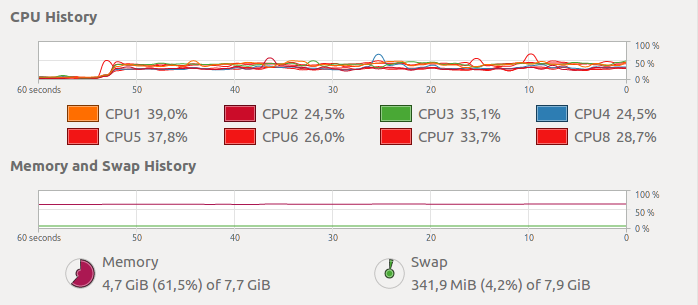
\includegraphics[width=100mm, keepaspectratio]{figures/tf_cpu}
\caption{A Tensorflownban id�tott logisztikus regresszi� er�forr�s ig�nye.} 
\label{fig:tf_cpu}
\end{figure}

Mint l�that� a scikit-learnben elind�tott futtat�s a teszt g�p �sszes mem�ri�j�t felem�sztette, illetve a magok kihaszn�l�sa is nagyon rossz volt, mind�ssze egyetlen magot haszn�lt ki. Ezzel szemben a Tensorflowban approxim�lt modell nagyon egyenletes magkihaszn�lts�g mellett minim�lis mem�ria ig�nnyel oldotta meg a feladatot. Term�szetesen nem �ll�tom hogy a k�t feladat identikus volt, mivel m�s algoritmusokkal jutottak el a v�geredm�nyig. Tov�bbi kutat�saimb�l kider�lt hogy ez a Scikit-learn alap�rtelmezett optimaliz�ci�s algoritmus�nak k�sz�nhet� amit a liblinear k�nyvt�r val�s�t meg. Amikor ezt kicser�ltem SAG megold�ra, akkor a g�p lefagy�s�nak probl�m�ja elt�nt, de m�g mindig konvergencia probl�m�k l�ptek fel. Az SAG egy kifejezetten �j fejlem�ny a numerikus optimaliz�ci� ter�let�n, amit egy 2013-as publik�ci� mutat be "Minimizing Finite Sums with Stochastic Average Gradient"\cite{sag}.
Ezen fel�l m�g megprob�ltam az adathalmazt a newton konjug�lt-gradiens m�dszerrel megtanulni. Ez is sikertelen lett az er�forr�sok hi�nya miatt. Ami �rthet�, hiszen egy gyors konvergenci�t ig�r, de m�g a sima liblinear megold�n�l is nagyobb er�forr�s ig�nnyel.

Ez a m�r�si sorozat �gy gondolom hogy egy�rtelm�en r�vil�g�t a numerikus optimaliz�ci� kiemelked� fontoss�g�ra a g�pi tanul�s applik�ci�kban. Az adathalmaz amin teszteltem a met�dusokat nem volt nagy, a CIFAR-10 mind�ssze 180 megabyte. Amennyiben ezeket a m�r�seket az akad�mia szerverein v�geztem volna el, akkor gond n�lk�l tan�thattam volna ak�rmelyik m�dszerrel. Viszont �gy, hogy a tesztrendszer is igen korl�tozott j�l megvil�g�totta a nagy adathalmazokon val� tanul�s egyik nagy probl�m�j�t. Hab�r a mostani szevereink m�r hatalmas er�forr�sokkal b�rnak a klasszikus m�dszereink amik folyamatosan az eg�sz adathalmazzal val� interakci�t ig�nylik, mint mondjuk az eredeti logisztikus regresszi� vagy svm tan�t� algoritmusok m�gsem lesznek haszn�lhat�ak egyszer�en az adathalmaz puszta nagys�ga miatt. Ez�rt is fontos hogy a mostani kutat�sok nagyr�sze a numerikus optmaliz�ci� ter�n a sztochatsztikus m�dszerekre koncentr�l amik v�letlenszer�en �sszev�logatott kis tan�t� halmazokkal approxim�lj�k a teljes adathalmaz tulajdons�gait.

//TODO: GPU

\section{A baseline eredm�nyek ismertet�se}
Mint m�r eml�tettem, k�t alap met�sdus amihez a saj�t eredm�nyeimet m�rtem a logsztikus regresszi�, �s egy egyszer� SVM volt, amihez polynomi�lis kernelt haszn�ltam 3 as foksz�mmal �s az els� rend� tagokat haszn�lva. Az eredm�nyeim az eredm�nyiemet az MNIST adathalmazon a \tabref{baselineMNIST}~t�bl�zat, �s a \tabref{baselineCIFAR}~t�bl�zat szeml�lteti.

\begin{table}[ht]
	\footnotesize
	\centering
	\caption{A baseline m�r�sek eremd�nye az MNIST adathalmaz nyers pixeljein, haszn�lt k�nyvt�r: Scikit-learn} \label{tab:baselineMNIST}
	\begin{tabular}{ | l | c |}
	\hline
	tanul� met�dus & Teszt halmaz hiba sz�zal�ka \\ \hline
	Logisztikus regresszi� & 8\%\\
	SVM poly kernel fok: 3 coef0: 1 &  6\%\\
	\hline
	\end{tabular}
\end{table}

Az MNIST-en el�rt eredm�nyek nem a legjobbak, de eg�szen optim�lis eredm�nyek ilyen egyszer� elj�r�sokkal is. Ezeken sokat lehet jav�tani a k�pek el�feldolgoz�s�val, de ez egy k�l�n szakdolgozat t�m�ja lehetne, �gyhogy ezzel most itt nem foglalkozok. Minden strukt�r�t a nyers adatokon kezdtem el tr�ningezni, klasszikus el�feldolgoz�si l�p�sek alkalmaz�sa n�lk�l. A teljess�g kedv��rt megeml�tem hogy a legjobb eredm�ny amit SVM-el �rtek el az MNIST adahalmazon annak a fel�p�t�se a k�vetkez� volt: \emph{Virtual SVM, deg-9 poly, 2-pixel jittered}, el�feldolgoz�si l�p�sk�nt csak kiegyenes�t�st haszn�lt (deskewing), az el�rt teszt hibasz�zal�k pedig \emph{0.56\%} volt.

\begin{table}[ht]
	\footnotesize
	\centering
	\caption{A baseline m�r�sek eremd�nye az CIFAR-10 adathalmaz nyers pixeljein, haszn�lt k�nyvt�r: Scikit-learn} \label{tab:baselineCIFAR}
	\begin{tabular}{ | l | c |}
	\hline
	tanul� met�dus & Teszt halmaz hiba sz�zal�ka \\ \hline
	Logisztikus regresszi� & 62\%\\
	Linear SVM with improved LCC & 26\%\\
	\hline
	\end{tabular}
\end{table}

Mint l�tni lehet itt ezek a met�dusok m�r k�zel sem teljes�tenek annyira f�nyesen. Az SVM-et nem �n futtattam le, mert ahhoz a teszt g�p nem volt el�g er�s. Az egy ICML 2010-es konferenci�n bemutatott eredm�ny volt, amit a "Improved Local Coordinate Coding using Local Tangents"\cite{svmCIFAR}-ban publik�ltak.

\section{Az MLP-vel elv�gzett m�r�seim eredm�nyei}

\subsection{Az MNIST m�r�sek}
A t�bbr�teg� perceptronokr�l ismeretes hogy a r�tegek k�z�tt teljes kapcsolat van, �s az adathalmaznak semmilyen tulajdons�g�t nem �p�tik bele az architekt�r�ba a priori, nem �gy mint a konvoluci�s h�l�zatok, ahol a transzl�ci�s invariancia el�re felt�telezett, �s maga a h�l�zat tartalmazza a k�nyszereket. Ez alappvet�en abban is megny�lv�nul hogy a h�l�zat nem egy h�rom dimenzi�s bemenetre (magass�g, sz�less�g, m�lys�g(RGB)) t�maszaszkodik, hanem egy egyszer� vektorra. Az MNIST-en el�rt eredm�nyeimet egy ilyen egyszer� strukt�r�val a \tabref{mnistMlpMeasurements}~t�bl�zat mutatja be, a m�r�seket a fejezet elej�n ismertetett tesztg�p CPU-j�n v�geztem. A bemenet egy 784 elem� vektor volt, ami praktikusan az MNIST adathalmaz egyetlen vektorba lap�tva sorr�l sorra.

\begin{table}[ht]
	\footnotesize
	\centering
	\caption{A saj�t MLP teljes�tm�nye az MNIST adathalmazon, 20 000 tan�t� batch ut�n. Bemenetek sz�ma: 784, reLu aktiv�ci�val, L2 reguraliz�ci�val, aminek az egy�tthat�ja 0.0005 vot. A s�lyokat csonkolt norm�l eloszl�ssal inicializ�ltam, standard sz�r�s: 0.1, k�z�p�rt�k: 0.0.} \label{tab:mnistMlpMeasurements}
	\begin{tabular}{ | l | c | c |}
	\hline
	neuron strukt�ra & Optimaliz�l� algoritmus & Teszt szet hiba sz�zal�k \\ \hline
	10 & SGD learning-rate: 0.5 & 8\%\\
	1024-10 & SGD learning-rate: 0.5 & 3.9\%\\
	400-10 & SGD learning-rate: 0.5 & 0.9\%\\
	400-10 & Adam & 0,9\%\\
	800-10 & Adam & 0.9\%\\
	800-10 & SGD learning-rate: 0.5 & 0.55\%\\
	\hline
	\end{tabular}
\end{table}

L�that� hogy az els� strukt�ra a logisztikus regresszi�val, ami nem meglep�, hiszen egy egyr�teg� strukt�ra softmax f�ggv�nnyel a v�g�n praktikusan ugyanakkora �ltal�nos�t� k�pess�ggel rendelkezik mint egy klasszikus m�dszerekkel tan�tott multinomi�lis logisztikus regresszor. Ezen az eredm�nyen l�nyegesen tudtam jav�tani miut�n hozz�adtam egy 1024 elem� rejtett r�teget, ami n�velte a h�l� �ltal�nos�t� k�pesseg�t, de 20'000 l�p�s alatt nem volt k�pes t�ltanul�s n�lk�l megtanulni a feladatot. Ahogyan cs�kkentettem a h�l�zat m�ret�t az cs�kkentette a t�ltanul�s m�rt�k�t �s jelent�s teljes�tm�ny n�veked�st hozott. A 0.9\%-os hiba eredm�ny m�r elmondhat� hogy eg�szen k�zel van az eddigi legjobb el�rt eredm�nyhez 1 rejtett r�teggel, ami 0.7\%. Azt v�rtam volna hogy az Adapt�v momentum k�zel�t� (adam) m�dszer jav�t a h�l�zat eredm�ny�n, de nem �gy lett. �ltal�ban az Adam optimaliz�tor el�nye abban rejlik hogy mivel a momentumot �s a tanul�si r�t�t adapt�van sz�m�tja minden batchre, ez�rt kevesebb hiperparam�tert kell �ll�tani. Ez term�szetesen megn�vekedett sz�m�t�s ig�nnyel szokott j�rni. A legjobb eredm�nyt az adathalmazon amit el�rtem az \emph{0.55\%} volt, ami m�r igen k�zel j�r a legjobb megold�shoz amit hasonl� h�l�zattal el�rtek.

A \figref{adamsSum}~�bra �s a \figref{sgdSum}~�bra mutatja hogy mekkora hat�ssal van az gradiens keres�si elj�r�s a megtanult s�lyokra. L�tszik hogy a k�t eredm�ny mer�ben m�s optimumra �llt be. Mint ahogyan a \tabref{MLPTablazat}~t�bl�ztb�l is l�tszik, az SGD-t haszn�l� h�l�zat sokkal k�zelebb ker�lt a teszt adathalmaz �ltal�nos k�p�hez. Az is nagyon j�l l�tszik a k�peken hogy az ADAM optimiz�tor �gy alak�totta a koefficienseket hogy l�nyegesen kissebb v�ltoztat�sokat tegyen a fel�leten, ez�rt egy�ltal�n nem ugr�lt annyira a s�lyok �rt�ke mint az SGD-n�l. Viszont mind a kett� a vesztes�gf�ggv�ny stabil�t�si pontj�t olyan 2000 iter�ci� ut�n �rte el, onnant�l m�r csak oszcill�ltak a marad�k 18000 l�p�sben.

\begin{figure}[!ht]
\centering
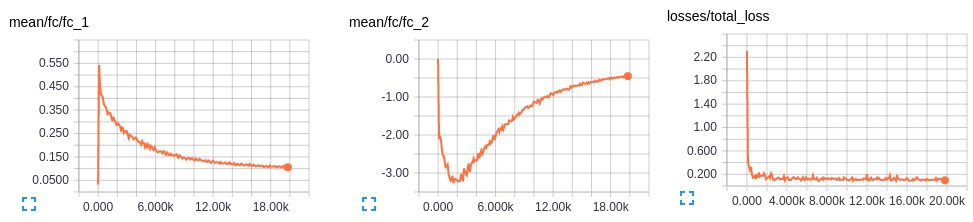
\includegraphics[width=150mm, keepaspectratio]{figures/adamSum}
\caption{A vesztes�gf�ggv�ny �s a h�l�zat s�ly �tlagainak a r�tegenk�nti alakul�sa ADAM optimiz�tor mellett.} 
\label{fig:adamsSum}
\end{figure}

\begin{figure}[!ht]
\centering
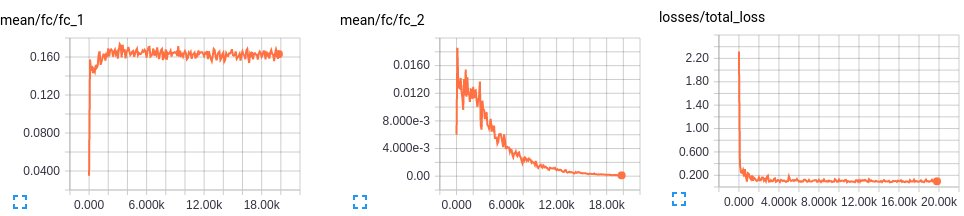
\includegraphics[width=150mm, keepaspectratio]{figures/sgdSum}
\caption{A vesztes�gf�ggv�ny �s a h�l�zat s�ly �tlagainak a r�tegenk�nti alakul�sa SGD optimiz�tor mellett.} 
\label{fig:sgdSum}
\end{figure}


\subsection{A CIFAR-10 m�r�sek}
Miut�n az mnist adathalmazon sikeres m�r�seket v�geztem eg�szen egyszer� MLP h�l�zatokkal kiv�ncsi lettem hogy ezek a h�l�zatok mennyire viszik �t a teljes�tm�ny�ket egy fokkal bonyolultabb adathalmazra. A k�t adathalmaz tulajdons�gai egym�shoz k�pest:

\begin{itemize}
\item Mindk�t adathalmaz 10 oszt�lyt tartalmaz.
\item Mindk�t adathalmaz 10'000 teszt k�pet tartalmaz, 1000-et oszt�lyonk�nt.
\item A CIFAR-10es adathalmaz 10'000-rel kevesebb tan�t� k�pet tartalmaz, ez oszt�lyonk�nt 1000 darab.
\item Am�g az MNIST 28x28as fekete feh�r k�peket tartalmazott, addig a CIFAR-10 32x32-es sz�nes k�peket tartalmaz.
\end{itemize}

Ami r�gt�n szembet�nik hogy am�g az MNIST 784 dimenzi�t tartalmazott, addig a CIFAR-10 egy 3072 dimenzi�s adathalmaz, teh�t az adathalmaz komplexit�sa ha csak tiszt�n a dimenzi�kat n�zz�k akkor a n�gyszeres�re n�tt. Ennek megfelel�en a h�l�zatok ha ugyanazokat a h�l�zatokat prob�ljuk haszn�lni, akkor drasztikus teljes�tm�ny cs�kken�st vagyunk k�nytelenek tapasztalni.

\begin{table}[ht]
	\footnotesize
	\centering
	\caption{A saj�t MLP teljes�tm�nye az CIFAR adathalmazon, 20 000 tan�t� batch ut�n. Bemenetek sz�ma: 3072, reLu aktiv�ci�val, L2 reguraliz�ci�val, aminek az egy�tthat�ja 0.0005 vot. A s�lyokat csonkolt norm�l eloszl�ssal inicializ�ltam, standard sz�r�s: 0.1, k�z�p�rt�k: 0.0.} \label{tab:MLPTablazat}
	\begin{tabular}{ | l | c | c |}
	\hline
	neuron strukt�ra & Optimaliz�l� algoritmus & Teszt szet hiba sz�zal�k \\ \hline
	10 & SGD learning-rate: 0.5 & 80\%\\
	10 & SGD learning-rate: 0.001 & 75\%\\
	400 - 10 & SGD learning-rate: 0.01 & 79 \%\\
	1024 - 10 & SGD learning-rate: 0.01 & 90\%\\
	\hline
	\end{tabular}
\end{table}

\subsection{Az el�tan�t�s eredm�nyeinek �sszefoglal�sa}
Arra a sz�momra meglep� eredm�nyre jutottam hogy az el�tan�t�s az az �n m�r�seim k�zben minden esetben csak rontott a h�l�zat klasszifik�ci�s teljes�tm�ny�n. Az �ltalam v�rt eredm�ny az lett volna, hogy az el�tan�t�s jelent�sen jav�tani fog a h�l�k teljes�tm�ny�n, f�leg nagy neuron sz�mn�l. A \tabref{mnistMlpPretrainedTable}~t�bl�zat �s a \tabref{cifarMlpPretrainedTable} t�bl�zat mutatja be az eredm�nyeimet.

\begin{table}[ht]
	\footnotesize
	\centering
	\caption{Az el�tan�tott MLP h�lozatok eredm�nye a MNIST adathalmazon, 25 elem� batchekkel.} \label{tab:mnistMlpPretrainedTable}
	\begin{tabular}{ | l | c | c | c |}
	\hline
	neuron strukt�ra & \parbox[c]{5cm}{nem-fel�gyelt/fel�gyelt\\epoch sz�m} & Optimaliz�l� algoritmus & \parbox[c]{5cm}{Teszt szet hiba sz�zal�k\\el�tan�t�ssa / n�lk�le} \\ \hline
	800 - 10 & 15/30 & SGD learning-rate: 0.05 & 92\% / 0.9\% \\
	500-500-2000-30 & 15/30 & learning-rate: 0.001 & 88,5\% / 3,2\% \\
	\hline
	\end{tabular}
\end{table}

\begin{table}[ht]
	\footnotesize
	\centering
	\caption{Az el�tan�tott MLP h�lozatok eredm�nye a CIFAR adathalmazon, 25 elem� batchekkel.} \label{tab:cifarMlpPretrainedTable}
	\begin{tabular}{ | l | c | c | c |}
	\hline
	neuron strukt�ra & \parbox[c]{5cm}{nem-fel�gyelt/fel�gyelt\\epoch sz�m} & Optimaliz�l� algoritmus & \parbox[c]{5cm}{Teszt szet hiba sz�zal�k\\el�tan�t�ssa / n�lk�le} \\ \hline
	400 - 10 & 10/10 & SGD learning-rate: 0.001 & 91\% / 55\% \\
	500-500-2000-30 & 10/10 & learning-rate: 0.001 & 88,5\% / 3,2\% \\
	\hline
	\end{tabular}
\end{table}

�gy magyar�zom ezeket az elszomor�t� eredm�nyeket hogy az el�tan�t�s k�vetkezt�ben egy rossz lok�lis minimumba ragadt be a h�l�, ahonnan nem tudodd kij�nni egyik esetben sem. Ahhoz hogy ezt a feltev�semet igazolja mmegn�ztem az mnist adathalmazon tan�tott nagym�ret� (500-500-2000-30 neuron) h�l�nak a vesztes�gf�ggv�ny�t �s a pontoss�g�nak a n�veked�s�t a valid�ci�s adathalmazon.
Ez el�tan�t�s n�lk�li h�l� m�rt eredm�nyei a \figref{bigDbnPretrained}~�br�n, az el�tan�t�ssal tan�tott h�l�na� pedig a \figref{bigDbnNotPretrained}~�br�n l�that�ak. Az �br�kon sz�pen kij�n hogy am�g az el�tan�t�s n�lk�li h�l� mindk�t m�rt�ket tenkintve egy viszonylag sima, egyenletes g�rb�t �r le, ami egy minimumhoz konverg�l, addig az el�tan�tott h�l� beragadt egy rossz lok�lis minimumba, ahonnan nem tud kiker�lni. Ebb�l azt sz�rtem le, hogy �rdekes m�don nem felt�tlen azok a j� jellemz�k oszt�lyoz�shoz, amik a rekonstrukci�hoz. Pedig nekem eg�szen intut�v lett volna, �s az irodalomban is sokat olvastam r�la hogy ez az el�nye az RBM-ekkel val� el�tan�t�snak.

\begin{figure}[!ht]
\centering
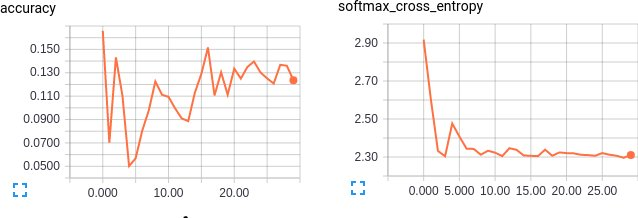
\includegraphics[width=100mm, keepaspectratio]{figures/bigDbnPretrained}
\caption{A 500-500-2000-30 neuron� el�tan�tott MLP vesztes�gf�ggv�ny�nek, �s a valid�ci�shalmazon val� pontoss�g�nak alakul�sa.} 
\label{fig:bigDbnPretrained}
\end{figure}

\begin{figure}[!ht]
\centering
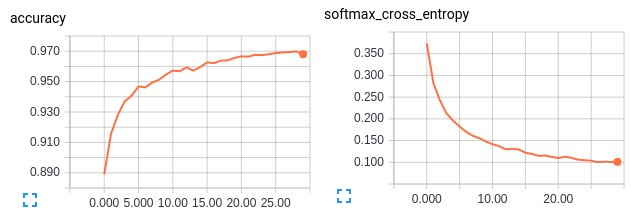
\includegraphics[width=100mm, keepaspectratio]{figures/bigDbnNotPretrained}
\caption{A 500-500-2000-30 neuron� \emph{nem} el�tan�tott MLP vesztes�gf�ggv�ny�nek, �s a valid�ci�shalmazon val� pontoss�g�nak alakul�sa.} 
\label{fig:bigDbnNotPretrained}
\end{figure}



\section{A konvoluci�s h�l�zatok eredm�nyei}
Miut�n l�thattuk hogy az MLP-k m�r nehezen b�rk�znak meg a CIFAR-10 komplexit�s� feladatokkal a figyelmemet az elm�leti r�szben oly sok helyet elfoglal� konvoluci�s architekt�r�k fel ford�tottam. Mivel ezek az architekt�r�k �rik el jelenleg a legjobb eredm�nyeket a neur�lis jelfeldolgoz�s sz�les ter�let�n, nem csak k�poszt�lyoz�sban hanem ak�r besz�dszintetiz�l�sban is, ez�rt nagy rem�nyekkel fordultam ezekhez a strukt�r�khoz. Az eredm�nyeimet a \tabref{CnnTablazat}~t�bl�zat mutatja. Az al�bbi felsorol�s az �ltalam haszn�lt h�l�zatokat �rja le.
\begin{itemize}
\item conv2d -> relu -> conv2d -> relu -> flatten -> softmax
\item conv2d -> relu -> maxpool\textunderscore 2x2 -> conv2d -> relu -> maxpool\textunderscore2x2 -> flatten -> fullyconnected -> dropout\textunderscore 0.5 -> softmax
\end{itemize}

\begin{table}[ht]
	\footnotesize
	\centering
	\caption{A saj�t MLP teljes�tm�nye az CIFAR adathalmazon, 20 000 tan�t� batch ut�n. Bemenetek sz�ma: 3072, reLu aktiv�ci�val, L2 reguraliz�ci�val, aminek az egy�tthat�ja 0.0005 vot. A s�lyokat csonkolt norm�l eloszl�ssal inicializ�ltam, standard sz�r�s: 0.1, k�z�p�rt�k: 0.0.} \label{tab:CnnTablazat}
	\begin{tabular}{ | l | c | c |}
	\hline
	A strukt�ra sorsz�ma & Optimaliz�l� algoritmus & Teszt szet hiba sz�zal�k \\ \hline
	1 & ADAM  & 8\%\\
	2 & SGD ADAM & 1.2\%\\
	\hline
	\end{tabular}
\end{table}

\section{A konvoluci�s �s az MLP a}

\section{A hibrid architekt�r�k eredm�nyei}
%----------------------------------------------------------------------------
\chapter{A \LaTeX-sablon haszn�lata}
%----------------------------------------------------------------------------
Ebben a fejezetben r�viden, implicit m�don bemutatjuk a sablon haszn�lat�nak m�dj�t, ami azt jelenti, hogy sablon haszn�lata ennek a dokumentumnak a forr�sk�dj�t tanulm�nyozva v�lik teljesen vil�goss�. Amennyiben a szoftver-keretrendszer telep�tve van, a sablon alkalmaz�sa �s a dolgozat szerkeszt�se \LaTeX-ben a sablon seg�ts�g�vel tapasztalataink szerint j�val hat�konyabb, mint egy WYSWYG (\emph{What You See is What You Get}) t�pus� sz�vegszerkeszt� eset�n (pl. Microsoft Word, OpenOffice).

%----------------------------------------------------------------------------
\section{C�mk�k �s hivatkoz�sok}
%----------------------------------------------------------------------------
A \LaTeX~dokumentumban c�mk�ket (\verb+\label+) rendelhet�nk �br�khoz, t�bl�zatokhoz, fejezetekhez, list�khoz, k�pletekhez stb. Ezekre a dokumentum b�rmely r�sz�ben hivatkozhatunk, a hivatkoz�sok automatikusan felold�sra ker�lnek.

A sablonban makr�kat defini�ltunk a hivatkoz�sok megk�nny�t�s�hez. Ennek megfelel�en minden �bra (\emph{figure}) c�mk�je \verb+fig:+ kulcssz�val kezd�dik, m�g minden t�bl�zat (\emph{table}), k�plet (\emph{equation}), fejezet (\emph{section}) �s lista (\emph{listing}) rendre a \verb+tab:+, \verb+eq:+, \verb+sect:+ �s \verb+listing:+ kulcssz�val kezd�dik, �s a kulcsszavak ut�n tetsz�legesen v�lasztott c�mke haszn�lhat�. Ha ezt a konvenci�t betartjuk, akkor az el�bbi objektumok sz�m�ra rendre a \verb+\figref+, \verb+\tabref+, \verb+\eqref+, \verb+\sectref+ �s \verb+\listref+ makr�kkal hivatkozhatunk. A makr�k param�tere a c�mke, amelyre hivatkozunk (a kulcssz� n�lk�l). Az �sszes eml�tett hivatkoz�st�pus, bele�rtve az \verb+\url+ kulcssz�val bevezetett web-hivatkoz�sokat is a  \verb+hyperref+\footnote{Seg�ts�g�vel a dokumentumban megjelen� hivatkoz�sok nem csak dinamikuss� v�lnak, de sz�nezhet�k is, b�vebbet err�l a csomag dokument�ci�j�ban tal�lunk. Ez egy�ttal egy p�lda l�bjegyzet �r�s�ra.} csomagnak k�sz�nhet�en akt�vak a legt�bb PDF-n�zeget�ben, r�juk kattintva a dokumentum megfelel� oldal�ra ugrik a PDF-n�z� vagy a megfelel� linket megnyitja az alap�rtelmezett b�ng�sz�vel. A \verb+hyperref+ csomag a kimeneti PDF-dokumentumba k�nyvjelz�ket is k�sz�t a tartalomjegyz�kb�l. Ez egy szint�n akt�v tartalomjegyz�k, amelynek elemeire kattintva a n�zeget� behozza a kiv�lasztott fejezetet.

%----------------------------------------------------------------------------
\section{�br�k �s t�bl�zatok}
%----------------------------------------------------------------------------
A k�peket PDFLaTeX eset�n a vesztes�gmentes PNG, valamint a vesztes�ges JPEG form�tumban �rdemes elmenteni. Az EPS (PostScript) vektorgrafikus k�pform�tum beilleszt�s�t a PDFLatex k�zvetlen�l nem t�mogatja. Ehelyett egy lehet�s�g 200 dpi, vagy ann�l nagyobb felbont�sban raszteriz�lni a k�pet, �s PNG form�tumban elmenteni. Az egyes k�pek m�rete �ltal�ban nem, de sok k�p eset�n a dokumentum �sszm�rete �gy m�r szignifik�ns is lehet. A dokumentumban felhaszn�lt k�pf�jlokat a dokumentum forr�sa mellett �rdemes tartani, archiv�lni, mivel ezek hi�ny�ban a dokumentum nem fordul �jra. Ha lehet, a vektorgrafikus k�peket vektorgrafikus form�tumban is �rdemes elmenteni az �jrafelhaszn�lhat�s�g (az �tszerkeszthet�s�g) �rdek�ben.

Kapcsol�si rajzok legt�bbsz�r kim�solhat�k egy vektorgrafikus programba (pl. CorelDraw) �s onnan nagyobb felbont�ssal raszteriz�lva kimenthat�k PNG form�tumban. Ugyanakkor kiv�l� �br�k k�sz�thet�k Microsoft Visio vagy hasonl� program haszn�lat�val is: Visio-b�l az �br�k k�zvetlen�l PNG-be is menthet�k.

Lehet�s�geink Matlab �br�k eset�n:
\begin{itemize}
	\item K�perny�lop�s (\emph{screenshot}) is elfogadhat� min�s�g� lehet a dokumentumban, de �ltal�ban jobb felbont�st is el lehet �rni m�s m�dszerrel.
	\item A Matlab �br�t a \verb+File/Save As+ opci�val lementhetj�k PNG form�tumban (ugyanaz itt is �rv�nyes, mint kor�bban, ez�rt nem javasoljuk).
	\item A Matlab �br�t az \verb+Edit/Copy figure+ opci�val kim�solhatjuk egy vektorgrafikus programba is �s onnan nagyobb felbont�ssal raszteriz�lva kimenthatj�k PNG form�tumban (nem javasolt).
	\item Javasolt megold�s: az �br�t a \verb+File/Save As+ opci�val EPS \emph{vektorgrafikus} form�tumban elmentj�k, PDF-be konvert�lva beillesztj�k a dolgozatba.
\end{itemize}
Az EPS k�p az \verb+epstopdf+ programmal\footnote{a kor�bban eml�tett \LaTeX-disztrib�ci�kban megtal�lhat�} konvert�lhat� PDF form�tumba. C�lszer� egy batch-f�jlt k�sz�teni az �sszes EPS �bra leford�t�s�ra az al�bbi m�don (ez Windows alatt m�k�dik).
\begin{lstlisting}[frame=single,float=!ht]
@echo off
for %%j in (*.eps) do (
echo converting file "%%j"
epstopdf "%%j"
)
echo done .
\end{lstlisting}

Egy ilyen parancsf�jlt (\verb+convert.cmd+) elhelyezt�k a sablon \verb+figures\eps+ k�nyvt�r�ba, �gy a felhaszn�l�nak csak annyi a dolga, hogy a \verb+figures\eps+ k�nyvt�rba kimenti az EPS form�tum� vektorgrafikus k�pet, majd lefuttatja a \verb+convert.cmd+ parancsf�jlt, ami PDF-be konvert�lja az EPS f�jlt.

Ezek ut�n a PDF-�br�t ugyan�gy lehet a dokumentumba beilleszteni, mint a PNG-t vagy a JPEG-et. A megold�s el�nye, hogy a leford�tott dokumentumban is vektorgrafikusan t�rol�dik az �bra, �gy a m�rete j�val kisebb, mintha raszteriz�ltuk volna beilleszt�s el�tt. Ez a m�dszer minden -- az EPS form�tumot ismer� -- vektorgrafikus program (pl. CorelDraw) eset�n is haszn�lhat�.

A k�pek beilleszt�s�re az \sectref{LatexTools}. fejezetben mutattunk be p�ld�t (\figref{TexnicCenter}~�bra). Az el�z� mondatban egy�ttal az automatikusan felold�d� �brahivatkoz�sra is l�thatunk p�ld�t. T�bb k�pf�jlt is beilleszthet�nk egyetlen �br�ba. Az egyes k�pek k�z�tti horizont�lis �s vertik�lis marg�t metrikusan szab�lyozhatjuk (\figref{HVSpaces}~�bra). Az �br�k elhelyez�s�t sz�mtalan tipogr�fiai szab�ly egyidej� teljes�t�s�vel a ford�t� maga v�gzi, a dokumentum �r�ja csak preferenci�it jelezheti a ford�t� fel� (olykor ez bossz�s�got is okozhat, ilyenkor pl. a k�p m�ret�vel lehet j�tszani).

\begin{figure}[!ht]
\centering
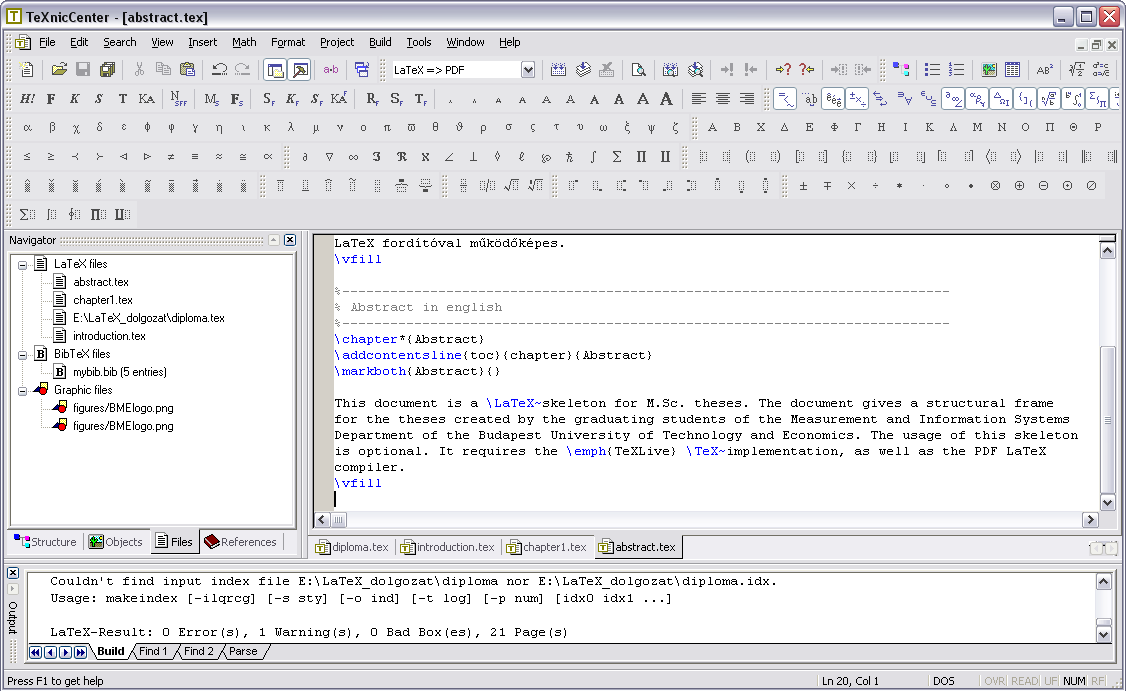
\includegraphics[width=67mm, keepaspectratio]{figures/TeXnicCenter.png}\hspace{1cm}
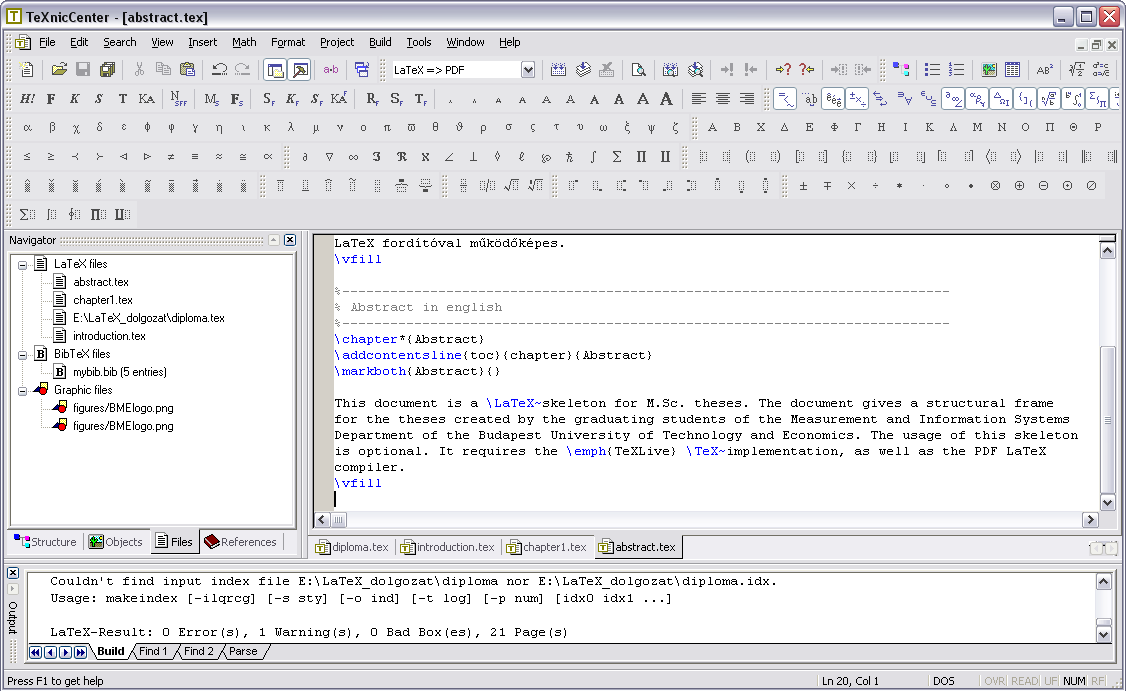
\includegraphics[width=67mm, keepaspectratio]{figures/TeXnicCenter.png}\\\vspace{5mm}
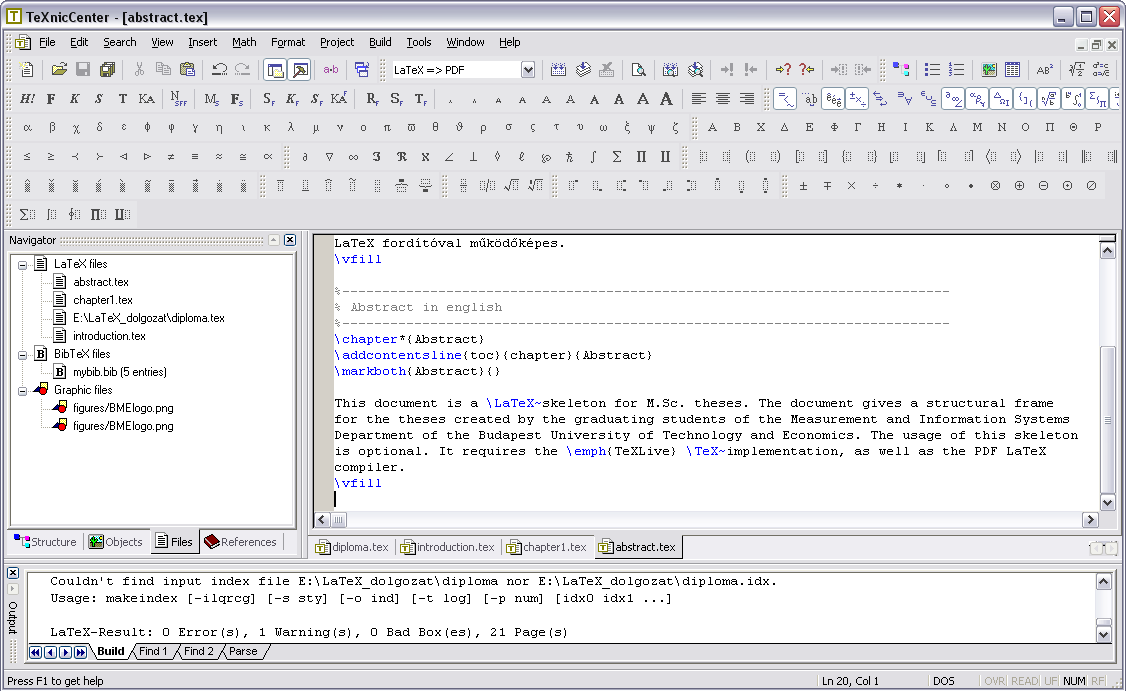
\includegraphics[width=67mm, keepaspectratio]{figures/TeXnicCenter.png}\hspace{1cm}
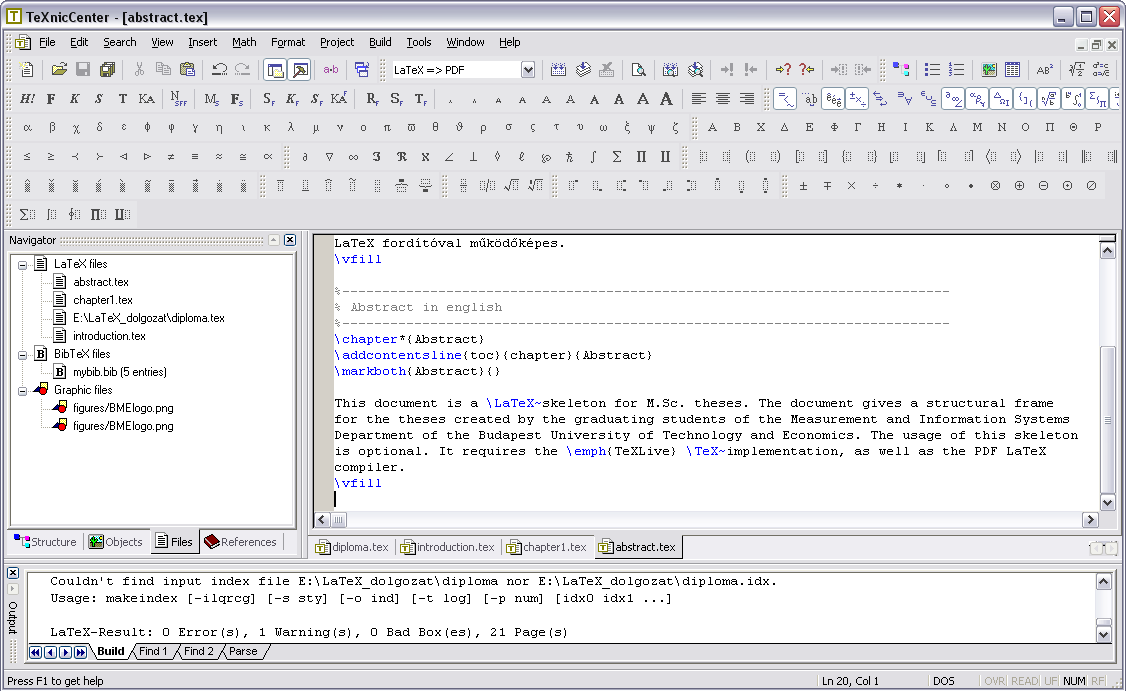
\includegraphics[width=67mm, keepaspectratio]{figures/TeXnicCenter.png}
\caption{T�bb k�pf�jl beilleszt�se eset�n t�rk�z�ket is �rdemes haszn�lni.} 
\label{fig:HVSpaces}
\end{figure}

A t�bl�zatok haszn�lat�ra a \tabref{TabularExample}~t�bl�zat mutat p�ld�t.
A t�bl�zat c�mk�je nem v�letlen�l ker�lt a t�bl�zat f�l�, ez a szokv�nyos.
\begin{table}[ht]
	\footnotesize
	\centering
	\caption{Az �rajel-gener�tor chip �rajel-kimenetei.} \label{tab:SysClocks}
	\begin{tabular}{ | l | c | c |}
	\hline
	�rajel & Frekvencia & C�l pin \\ \hline
	CLKA & 100 MHz & FPGA CLK0\\
	CLKB & 48 MHz  & FPGA CLK1\\
	CLKC & 20 MHz  & Processzor\\
	CLKD & 25 MHz  & Ethernet chip \\
	CLKE & 72 MHz  & FPGA CLK2\\
	XBUF & 20 MHz  & FPGA CLK3\\
	\hline
	\end{tabular}
	\label{tab:TabularExample}
\end{table}


%----------------------------------------------------------------------------
\section{Felsorol�sok �s list�k}
%----------------------------------------------------------------------------
Sz�mozatlan felsorol�sra mutat p�ld�t a jelenlegi bekezd�s:
\begin{itemize}
	\item \emph{els� bajusz:} ide lehetne �rni az els� elem kifej�s�t,
	\item \emph{m�sodik bajusz:} ide lehetne �rni a m�sodik elem kifej�s�t,
	\item \emph{ez meg egy szak�ll:} ide lehetne �rni a harmadik elem kifej�s�t.
\end{itemize}

Sz�mozott felsorol�st is k�sz�thet�nk az al�bbi m�don:
\begin{enumerate}
	\item \emph{els� bajusz:} ide lehetne �rni az els� elem kifej�s�t, �s ez a kifejt�s �gy n�z ki, ha t�bb sorosra sikeredik,
	\item \emph{m�sodik bajusz:} ide lehetne �rni a m�sodik elem kifej�s�t,
	\item \emph{ez meg egy szak�ll:} ide lehetne �rni a harmadik elem kifej�s�t.
\end{enumerate}
A felsorol�sokban sorok v�g�n vessz�, az utols� sor v�g�n pedig pont a szok�sos �r�sjel. Ez al�l kiv�telt k�pezhet, ha az egyes elemek t�bb teljes mondatot tartalmaznak.

List�kban a dolgozat sz�veg�t�l elk�l�n�tend� k�dr�szleteket, programsorokat, pszeudo-k�dokat jelen�thet�nk meg (\listref{Example}~lista). 
\begin{lstlisting}[frame=single,float=!ht,caption=A fenti sz�mozott felsorol�s \LaTeX- forr�sk�dja, label=listing:Example]
\begin{enumerate}
	\item \emph{els� bajusz:} ide lehetne �rni az els� elem kifej�s�t, 
	�s ez a kifejt�s �gy n�z ki, ha t�bb sorosra sikeredik,
	\item \emph{m�sodik bajusz:} ide lehetne �rni a m�sodik elem kifej�s�t,
	\item \emph{ez meg egy szak�ll:} ide lehetne �rni a harmadik elem kifej�s�t.
\end{enumerate}
\end{lstlisting}
A lista keret�t, h�tt�rsz�n�t, eg�sz st�lus�t megv�laszthatjuk. R�ad�sul k�l�nf�le programnyelveket �s a nyelveken bel�l kulcsszavakat is defini�lhatunk, ha sz�ks�ges. Err�l b�vebbet a \verb+listings+ csomag hivatalos le�r�s�ban tal�lhatunk.

%----------------------------------------------------------------------------
\section{K�pletek}
%----------------------------------------------------------------------------
Ha egy formula nem t�ls�gosan hossz�, �s nem akarjuk hivatkozni a sz�vegb�l, mint p�ld�ul a $e^{i\pi}+1=0$ k�plet, \emph{sz�vegk�zi k�pletk�nt} szok�s le�rni. Csak, hogy m�sik p�ld�t is l�ssunk, az $U_i=-d\Phi/dt$ Faraday-t�rv�ny a $\rot E=-\frac{dB}{dt}$ differenci�lis alakban adott Maxwell-egyenlet fel�letre vett integr�lj�b�l vezethet� le. L�that�, hogy a \LaTeX-ford�t� a sork�z�ket betartja, �gy a sz�veg szed�se eszt�tikus marad sz�vegk�zi k�pletek haszn�lata eset�n is.

K�pletek eset�n az �ltal�nos konvenci�, hogy a kisbet�k skal�rt, a kis f�lk�v�r bet�k ($\mathbf{v}$) oszlopvektort -- �s ennek megfelel�en $\mathbf{v}^T$ sorvektort -- a kapit�lis f�lk�v�r bet�k ($\mathbf{V}$) m�trixot jel�lnek. Ha ett�l el szeretn�nk t�rni, akkor az alkalmazni k�v�nt jel�l�sm�dot c�lszer� k�l�n alfejezetben defini�lni. Ennek megfelel�en, amennyiben $\mathbf{y}$ jel�li a m�r�sek vektor�t, $\mathbf{\vartheta}$ a param�terek vektor�t �s $\hat{\mathbf{y}}=\mathbf{X}\vartheta$ a param�terekben line�ris modellt, akkor a \emph{Least-Squares} �rtelemben optim�lis param�terbecsl� $\hat{\mathbf{\vartheta}}_{LS}=(\mathbf{X}^T\mathbf{X})^{-1}\mathbf{X}^T\mathbf{y}$ lesz.

Emellett kiemelt, sorsz�mozott k�pleteket is megadhatunk, enn�l az \verb+equation+ �s a \verb+eqnarray+ k�rnyezetek helyett a korszer�bb \verb+align+ k�rnyezet alkalmaz�s�t javasoljuk (t�bb okb�l, k�l�nf�le probl�m�k elker�l�se v�gett, amelyekre most nem t�r�nk ki). Teh�t
\begin{align}
\dot{\mathbf{x}}&=\mathbf{A}\mathbf{x}+\mathbf{B}\mathbf{u},\\
\mathbf{y}&=\mathbf{C}\mathbf{x},
\end{align}
ahol $\mathbf{x}$ az �llapotvektor, $\mathbf{y}$ a m�r�sek vektora �s $\mathbf{A}$, $\mathbf{B}$ �s $\mathbf{C}$ a rendszert le�r� param�term�trixok. Figyelj�k meg, hogy a k�t egyenletben az egyenl�s�gjelek egym�shoz igaz�tva jelennek meg, mivel a mindkett�t az \& karakter el�zi meg a k�dban. Lehet�s�g van sz�mozatlan kiemelt k�plet haszn�lat�ra is, p�ld�ul
\begin{align}
\dot{\mathbf{x}}&=\mathbf{A}\mathbf{x}+\mathbf{B}\mathbf{u},\nonumber\\
\mathbf{y}&=\mathbf{C}\mathbf{x}\nonumber.
\end{align}
M�trixok fel�r�s�ra az $\mathbf{A}\mathbf{x}=\mathbf{b}$ inhomog�n line�ris egyenlet r�szletes kifejt�s�vel mutatunk p�ld�t:
\begin{align}
\begin{bmatrix}
a_{11} & a_{12} & \dots & a_{1n}\\
a_{21} & a_{22} & \dots & a_{2n}\\
\vdots & \vdots & \ddots & \vdots\\
a_{m1} & a_{m2} & \dots & a_{mn}
\end{bmatrix}
\begin{pmatrix}x_1\\x_2\\\vdots\\x_n\end{pmatrix}=
\begin{pmatrix}b_1\\b_2\\\vdots\\b_m\end{pmatrix}.
\end{align}
A \verb+\frac+ utas�t�s hat�konys�g�t egy �ltal�nos m�sodfok� tag �tviteli f�ggv�ny�n kereszt�l mutatjuk be, azaz
\begin{align}
W(s)=\frac{A}{1+2T\xi s+s^2T^2}.
\end{align}
A matematikai m�d minden szimb�lum�nak �s k�pess�g�nek a bemutat�s�ra term�szetesen itt nincs lehet�s�g, de gyors referenciak�nt hat�konyan haszn�lhat�k a k�vetkez� linkek:\\
\indent\url{http://www.artofproblemsolving.com/LaTeX/AoPS_L_GuideSym.php},\\
\indent\url{http://www.ctan.org/tex-archive/info/symbols/comprehensive/symbols-a4.pdf},\\
\indent\url{ftp://ftp.ams.org/pub/tex/doc/amsmath/short-math-guide.pdf}.\\
Ez pedig itt egy magyar�zat, hogy mi�rt �rdemes \verb+align+ k�rnyezetet haszn�lni:\\
\indent\url{http://texblog.net/latex-archive/maths/eqnarray-align-environment/}.

%----------------------------------------------------------------------------
\section{Irodalmi hivatkoz�sok}\label{sect:HowtoReference}
%----------------------------------------------------------------------------
Egy \LaTeX dokumentumban az irodalmi hivatkoz�sok defin�ci�j�nak k�t m�dja van. Az egyik a \verb+\thebibliograhy+ k�rnyezet haszn�lata a dokumentum v�g�n, az \verb+\end{document}+ lez�r�s el�tt.
\begin{lstlisting}[frame=single,float=!ht]
\begin{thebibliography}{9}

\bibitem{Lamport94} Leslie Lamport, \emph{\LaTeX: A Document Preparation System}. 
Addison Wesley, Massachusetts, 2nd Edition, 1994.

\end{thebibliography}
\end{lstlisting}

Ezek ut�n a dokumentumban a \verb+\cite{Lamport94}+ utas�t�ssal hivatkozhatunk a forr�sra. A fenti megad�s viszonylag k�tetlen, a szerz� maga form�zza az irodalomjegyz�ket. 

Egy sokkal professzion�lisabb m�dszer a BiB\TeX~haszn�lata, ez�rt ez a sablon is ezt t�mogatja. Ebben az esetben egy k�l�n sz�veges adatb�zisban defini�ljuk a forr�smunk�kat, �s egy k�l�n st�lusf�jl hat�rozza meg az irodalomjegyz�k kin�zet�t. Ez, �sszhangban azzal, hogy k�l�n form�tumkonvenci� hat�rozza meg a foly�irat-, a k�nyv-, a konferenciacikk- stb. hivatkoz�sok kin�zet�t az irodalomjegyz�kben (a sablon haszn�lata eset�n ezzel nem is kell foglalkoznia a hallgat�nak, de az eredm�nyt c�lszer� ellen�rizni). A felhaszn�lt hivatkoz�sok adatb�zisa egy \verb+.bib+ kiterjeszt�s� sz�veges f�jl, amelynek szerkezet�t a \listref{Bibtex} k�dr�szlet demonstr�lja. A forr�smunk�k bevitelekor a sor v�gi vessz�k k�l�n figyelmet ig�nyelnek, mert hi�nyuk a BiB\TeX-ford�t� hiba�zenet�t eredm�nyezi. A forr�smunk�kat t�pus szerinti kulcssz� vezeti be (\verb+@book+ k�nyv, \verb+@inproceedings+ konferenciakiadv�nyban megjelent cikk, \verb+@article+ foly�iratban megjelent cikk, \verb+@techreport+ valamelyik egyetem gondoz�s�ban megjelent m�szaki tanulm�ny, \verb+@manual+ m�szaki dokument�ci� eset�n stb.). Nemcsak a megjelen�s st�lusa, de a k�telez�en megadand� mez�k is t�pusr�l-t�pusra v�ltoznak. Egy j�l haszn�lhat� referencia a \url{http://en.wikipedia.org/wiki/BibTeX} oldalon tal�lhat�.
\begin{lstlisting}[frame=single,float=!ht,caption=P�lda sz�veges irodalomjegyz�k-adatb�zisra BiBTeX haszn�lata eset�n., label=listing:Bibtex]
@BOOK{Wettl04,
  author="Ferenc Wettl and Gyula Mayer and P�ter Szab�",
  title="\LaTeX~k�zik�nyv",
  publisher="Panem K�nyvkiad�",
  year=2004
}
@ARTICLE{Candy86,
  author ="James C. Candy",
  title  ="Decimation for Sigma Delta Modulation",
  journal="{IEEE} Trans.\ on Communications",
  volume =34,
  number =1,
  pages  ="72--76",
  month  =jan,
  year   =1986,
}
@INPROCEEDINGS{Lee87,
  author =       "Wai L. Lee and Charles G. Sodini",
  title =        "A Topology for Higher Order Interpolative Coders",
  booktitle =    "Proc.\ of the IEEE International Symposium on 
  Circuits and Systems",
  year =         1987,
  vol =          2,
  month =        may # "~4--7",
  address =      "Philadelphia, PA, USA",
  pages =        "459--462"
}
@PHDTHESIS{KissPhD,
  author =   "Peter Kiss",
  title =    "Adaptive Digital Compensation of Analog Circuit Imperfections 
  for Cascaded Delta-Sigma Analog-to-Digital Converters",
  school =   "Technical University of Timi\c{s}oara, Romania",
  month =    apr,
  year =     2000
}
@MANUAL{Schreier00,
  author = "Richard Schreier",
  title  = "The Delta-Sigma Toolbox v5.2",
  organization = "Oregon State University",
  year   = 2000,
  month  = jan,
  note   ="\newline URL: http://www.mathworks.com/matlabcentral/fileexchange/"
}
@MISC{DipPortal,
	author="Budapesti {M}�szaki �s {G}azdas�gtudom�nyi {E}gyetem 
	{V}illamosm�rn�ki �s {I}nformatikai {K}ar",
  title="{D}iplomaterv port�l (2011 febru�r 26.)",
  howpublished="\url{http://diplomaterv.vik.bme.hu/}",
}}
\end{lstlisting}

A st�lusf�jl egy \verb+.sty+ kiterjeszt�s� f�jl, de ezzel l�nyeg�ben nem kell foglalkozni, mert vannak be�p�tett st�lusok, amelyek j�l haszn�lhat�k. Ez a sablon a BiB\TeX-et haszn�lja, a hozz� tartoz� adatb�zisf�jl a \verb+mybib.bib+ f�jl. Megfigyelhet�, hogy az irodalomjegyz�ket a dokumentum v�g�re (a \verb+\end{document}+ utas�t�s el�) beillesztett \verb+\bibliography{mybib}+ utas�t�ssal hozhatjuk l�tre, a st�lus�t pedig ugyanitt a  \verb+\bibliographystyle{plain}+ utas�t�ssal adhatjuk meg. Ebben az esetben a \verb+plain+ el�re defini�lt st�lust haszn�ljuk (a sablonban is ezt �ll�tottuk be). A \verb+plain+ st�luson k�v�l term�szetesen sz�mtalan m�s el�re defini�lt st�lus is l�tezik. Mivel a \verb+.bib+ adatb�zisban ezeket megadtuk, a BiB\TeX-ford�t� is meg tudja k�l�nb�ztetni a szerz�t a c�mt�l �s a kiad�t�l, �s ez alapj�n automatikusan gener�l�dik az irodalomjegyz�k a st�lusf�jl �ltal meghat�rozott st�lusban.

Az egyes forr�smunk�kra a sz�vegb�l tov�bbra is a \verb+\cite+ paranccsal tudunk hivatkozni, �gy a \listref{Bibtex} k�dr�szlet eset�n a hivatkoz�sok rendre \verb+\cite{Wettl04}+, \verb+\cite{Candy86}+, \verb+\cite{Lee87}+, \verb+\cite{KissPhD}+, \verb+\cite{Schreirer00}+ �s \verb+\cite{DipPortal}+. Az irodalomjegyz�kben alap�rtelmez�sben csak azok a forr�smunk�k jelennek meg, amelyekre tal�lhat� hivatkoz�s a sz�vegben, �s ez �gy alapvet�en helyes is, hiszen olyan forr�smunk�kat nem illik az irodalomjegyz�kbe �rni, amelyekre nincs hivatkoz�s.

Mivel a ford�t�si folyamat sor�n t�bb l�p�sben old�dnak fel a szimb�lumok, ez�rt gyakran t�bbsz�r (TeXLive �s TeXnicCenter eset�n 2-3-szor) is le kell ford�tani a dokumentumot. Ilyenkor ez els� 1-2 ford�t�s esetleg szimb�lum-felold�sra vonatkoz� figyelmeztet� �zenettel z�rul. Ha hiba�zenettel z�rul b�rmelyik ford�t�s, akkor nincs �rtelme megism�telni, hanem a hib�t kell megkeresni. A \verb+.bib+ f�jl megv�ltoztat�skor sokszor nincs hat�sa a v�ltoztat�snak azonnal, mivel nem mindig fut �jra a BibTeX ford�t�. Ez�rt c�lszer� a v�ltoztat�s ut�n azt manu�lisan is lefuttatni (TeXnicCenter eset�n \verb+Build/BibTeX+).

Hogy a sz�vegbe �gyazott hivatkoz�sok kin�zet�t demonstr�ljuk, itt most sorban meghivatkozzuk a \cite{Wettl04}, \cite{Candy86}, \cite{Lee87}, \cite{KissPhD} �s az \cite{Schreier00} forr�smunk�t, valamint az \cite{DipPortal} weboldalt.

Megjegyzend�, hogy az �kezetes magyar bet�ket is tartalmaz� \verb+.bib+ f�jl az \verb+inputenc+ csomaggal bet�lt�tt \verb+latin2+ bet�k�szlet miatt ford�that�. Ugyanez a \verb+.bib+ f�jl hiba�zenettel fordul egy olyan dokumentumban, ami nem tartalmazza a \verb+\usepackage[latin2]{inputenc}+ sort. Speci�lis ig�ny eset�n az irodalmi adatb�zis �ltal�nosabb �rv�ny�v� tehet�, ha az �kezetes bet�ket speci�lis latex karakterekkel helyettes�tj�k a \verb+.bib+ f�jlban, pl. � helyett \verb+\'{a}+-t vagy � helyett \verb+\H{o}+-t �runk. 

Oldalt�r�s k�vetkezik (ld. forr�s).
\newpage

%----------------------------------------------------------------------------
\section{A dolgozat szerkezete �s a forr�sf�jlok}
%----------------------------------------------------------------------------
A diplomatervsablon (a kari ir�nyelvek szerint) az al�bbi f� fejezetekb�l �ll:
\begin{enumerate}
	\item 1 oldalas \emph{t�j�koztat�} a szakdolgozat/diplomaterv szerkezet�r�l (\verb+guideline.tex+), ami a v�gs� dolgozatb�l t�rlend�,
	\item \emph{feladatki�r�s} (\verb+project.tex+), a dolgozat nyomtatott verz�j�ban ennek a hely�re ker�l a tansz�k �ltal kiadott, a tansz�kvezet� �ltal al��rt feladatki�r�s, a dolgozat elektronikus verzi�j�ba pedig a feladatki�r�s egy�ltal�n ne ker�lj�n bele, azt k�l�n t�lti fel a tansz�k a diplomaterv-honlapra,
	\item \emph{c�moldal} (\verb+titlepage.tex+),
	\item \emph{tartalomjegyz�k} (\verb+diploma.tex+),
	\item a diplomatervez� \emph{nyilatkozat}a az �n�ll� munk�r�l (\verb+declaration.tex+),
	\item 1-2 oldalas tartalmi \emph{�sszefoglal�} magyarul �s angolul, illetve elk�sz�thet� m�g tov�bbi nyelveken is (\verb+abstract.tex+),
	\item \emph{bevezet�s}: a feladat �rtelmez�se, a tervez�s c�lja, a feladat indokolts�ga, a diplomaterv fel�p�t�s�nek r�vid �sszefoglal�sa (\verb+introduction.tex+),
	\item sorsz�mmal ell�tott \emph{fejezetek}: a feladatki�r�s pontos�t�sa �s r�szletes elemz�se, el�zm�nyek (irodalomkutat�s, hasonl� alkot�sok), az ezekb�l levonhat� k�vetkeztet�sek, a tervez�s r�szletes le�r�sa, a d�nt�si lehet�s�gek �rt�kel�se �s a v�lasztott megold�sok indokl�sa, a megtervezett m�szaki alkot�s �rt�kel�se, kritikai elemz�se, tov�bbfejleszt�si lehet�s�gek (\verb+chapter{1,2..n}.tex+),
	\item esetleges \emph{k�sz�netnyilv�n�t�s}ok (\verb+acknowledgement.tex+),
	\item r�szletes �s pontos \emph{irodalomjegyz�k} (ez a sablon eset�ben automatikusan gener�l�dik a \verb+diploma.tex+ f�jlban elhelyezett \verb+\bibliography+ utas�t�s hat�s�ra, a \sectref{HowtoReference}. fejezetben le�rtak szerint),
	\item \emph{f�ggel�kek} (\verb+appendices.tex+).
\end{enumerate}

A sablonban a fejezetek a \verb+diploma.tex+ f�jlba vannak beillesztve \verb+\include+ utas�t�sok seg�ts�g�vel. Lehet�s�g van arra, hogy csak az �ppen szerkeszt�s alatt �ll� \verb+.tex+ f�jlt ford�tsuk le, ezzel ler�vid�tve a ford�t�si folyamatot. Ezt a lehet�s�get az al�bbi k�dr�szlet biztos�tja a \verb+diploma.tex+ f�jlban.
\begin{lstlisting}[frame=single,float=!ht]
\includeonly{
	guideline,%
	project,%
	titlepage,%
	declaration,%
	abstract,%
	introduction,%
	chapter1,%
	chapter2,%
	chapter3,%
	acknowledgement,%
	appendices,%
}
\end{lstlisting}

Ha az al�bbi k�dr�szletben az egyes sorokat a \verb+%+ szimb�lummal kikommentezz�k, akkor a megfelel� \verb+.tex+ f�jl nem fordul le. Az oldalsz�mok �s a tartalomjegy�k term�szetesen csak akkor billennek helyre, ha a teljes dokumentumot leford�tjuk.

%----------------------------------------------------------------------------
\newpage
\section{Alapadatok megad�sa}
%----------------------------------------------------------------------------
A diplomaterv alapadatait (c�m, szerz�, konzulens, konzulens titulusa) a \verb+diploma.tex+ f�jlban lehet megadni az al�bbi k�dr�szlet m�dos�t�s�val.
\begin{lstlisting}[frame=single,float=!ht]
\newcommand{\vikszerzo}{B�dis-Szomor� Andr�s}
\newcommand{\vikkonzulens}{dr.~Konzulens Elem�r}
\newcommand{\vikcim}{Elektronikus terel�k}
\newcommand{\viktanszek}{M�r�stechnika �s Inform�ci�s Rendszerek Tansz�k}
\newcommand{\vikdoktipus}{Diplomaterv}
\newcommand{\vikdepartmentr}{B�dis-Szomor� Andr�s}
\end{lstlisting}

%----------------------------------------------------------------------------
\section{�j fejezet �r�sa}
%----------------------------------------------------------------------------
A f�fejezetek k�l�n \verb+chapter{1..n}.tex+ f�jlban foglalnak helyet. A sablonhoz 3 fejezet k�sz�lt. Tov�bbi f�fejezeteket �gy hozhatunk l�tre, ha �j \verb+chapter{i}.tex+ f�jlt k�sz�t�nk a fejezet sz�m�ra, �s a \verb+diploma.tex+ f�jlban, a \verb+\include+ �s \verb+\includeonly+ utas�t�sok argumentum�ba felvessz�k az �j \verb+.tex+ f�jl nev�t.






%----------------------------------------------------------------------------
\chapter*{K�sz�netnyilv�n�t�s}\addcontentsline{toc}{chapter}{K�sz�netnyilv�n�t�s}
%----------------------------------------------------------------------------

Ez nem k�telez�, ak�r t�r�lhet� is. Ha a szerz� sz�ks�g�t �rzi, itt lehet k�sz�netet nyilv�n�tani azoknak, akik hozz�j�rultak munk�jukkal ahhoz, hogy a hallgat� a szakdolgozatban vagy diplomamunk�ban le�rt feladatokat sikeresen elv�gezze. A konzulensnek val� k�sz�netnyilv�n�t�s sem k�telez�, a konzulensnek hivatalosan is dolga, hogy a hallgat�t konzult�lja.

%\listoffigures\addcontentsline{toc}{chapter}{�br�k jegyz�ke}
%\listoftables\addcontentsline{toc}{chapter}{T�bl�zatok jegyz�ke}

\bibliography{mybib}
\addcontentsline{toc}{chapter}{Irodalomjegyz�k}
\bibliographystyle{plain}

%----------------------------------------------------------------------------
\appendix
%----------------------------------------------------------------------------
\chapter*{F�ggel�k}\addcontentsline{toc}{chapter}{F�ggel�k}
\setcounter{chapter}{6}  % a fofejezet-szamlalo az angol ABC 6. betuje (F) lesz
\setcounter{equation}{0} % a fofejezet-szamlalo az angol ABC 6. betuje (F) lesz
\numberwithin{equation}{section}
\numberwithin{figure}{section}
\numberwithin{lstlisting}{section}
%\numberwithin{tabular}{section}

%----------------------------------------------------------------------------
\section{A TeXnicCenter fel�lete}
%----------------------------------------------------------------------------
\begin{figure}[!ht]
\centering
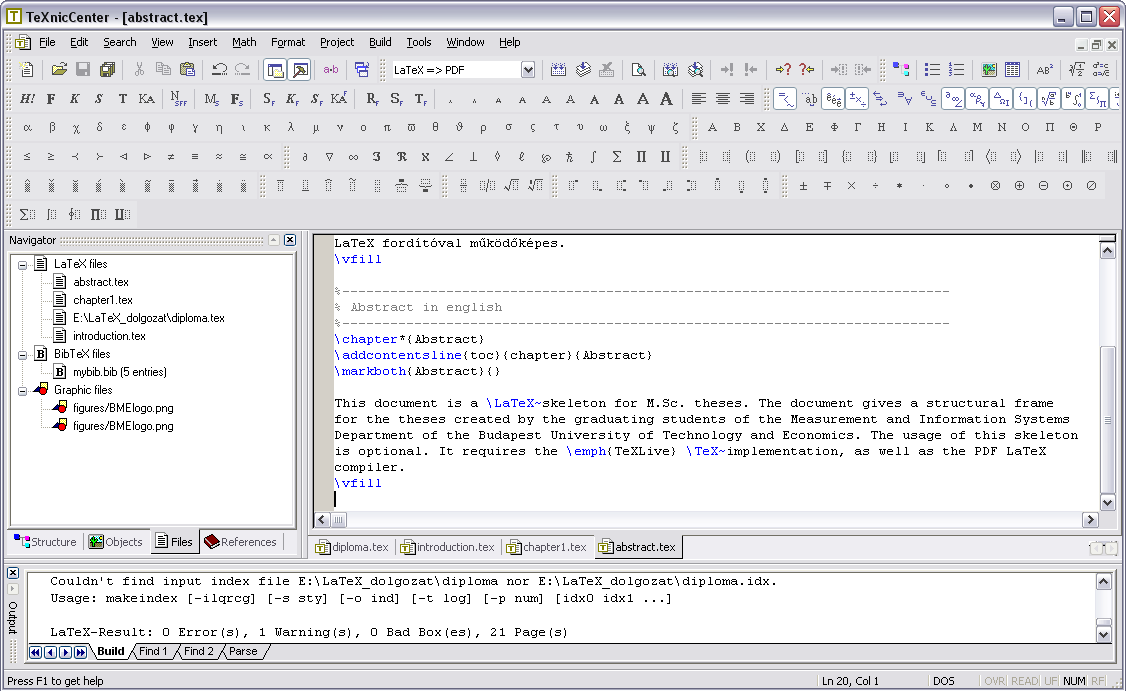
\includegraphics[width=150mm, keepaspectratio]{figures/TeXnicCenter.png}
\caption{A TeXnicCenter Windows alap� \LaTeX-szerkeszt�.} 
\end{figure}

%----------------------------------------------------------------------------
\clearpage\section{V�lasz az ,,�let, a vil�gmindens�g, meg minden'' k�rd�s�re}
%----------------------------------------------------------------------------
A Pitagorasz-t�telb�l levezetve
\begin{align}
c^2=a^2+b^2=42.
\end{align}
A Faraday-indukci�s t�rv�nyb�l levezetve
\begin{align}
\rot E=-\frac{dB}{dt}\hspace{1cm}\longrightarrow \hspace{1cm}
U_i=\oint\limits_\mathbf{L}{\mathbf{E}\mathbf{dl}}=-\frac{d}{dt}\int\limits_A{\mathbf{B}\mathbf{da}}=42.
\end{align}







\label{page:last}
\end{document}
